%------------------------------------------------------------------------------
% Template file for the submission of papers to IUCr journals in LaTeX2e
% using the iucr document class
% Copyright 1999-2003 International Union of Crystallography
% Version 1.2 (11 December 2002)
%------------------------------------------------------------------------------

\documentclass[preprint]{iucr}              % DO NOT DELETE THIS LINE
%\documentclass{article}
\usepackage{lscape}
\usepackage[centertags]{amsmath}
\usepackage{amsfonts}
\usepackage{amssymb}
\usepackage{amsthm}
\newcommand{\mb}[1]{\ensuremath{\mbox{\boldmath $ #1 $}}}
\newcommand{\mbss}[1]{\ensuremath{\mbox{\boldmath $ \scriptstyle #1 $}}}
\newcommand{\av}[1]{\ensuremath{\langle #1 \rangle}}
\newcommand{\dubint}{\int\!\!\!\int}
\newcommand{\intZ}{\int\!\!\!\int}
     %-------------------------------------------------------------------------
     % Information about the type of paper
     %-------------------------------------------------------------------------
     \paperprodcode{a000000}      % Replace with production code if known
     \paperref{xx9999}            % Replace xx9999 with reference code if known
     \papertype{FA}               % Indicate type of article
                                  %   FA - research papers (full article)
                                  %   SC - short communications
                                  %   FC - fast communications
                                  %   LA - lead article
                                  %   TR - topical review
                                  %   XL - crystallization papers
                                  % (Following categories rarely in LaTeX)
                                  %   AA - abstracts
                                  %   AD - addenda and errata
                                  %   AI - inorganic compounds
                                  %   AM - metal-organic compounds
                                  %   AO - organic compounds
                                  %   BC - books received
                                  %   BR - book reviews
                                  %   BI - biography
                                  %   CA - cif applications
                                  %   CD - crystal data
                                  %   CE - current events
                                  %   CI - inorganic compounds
                                  %   CL - calendar of events
                                  %   CM - metal-organic compounds
                                  %   CN - cryocrystallography papers
                                  %   CO - organic compounds
                                  %   CP - computer programs
                                  %   CR - crystallographers
                                  %   CS - scientific comment
                                  %   ED - editorial
                                  %   EI - inorganic compounds
                                  %   EM - metal-organic compounds
                                  %   EO - organic compounds
                                  %   FI - inorganic compounds
                                  %   FM - metal-organic compounds
                                  %   FO - organic compounds
                                  %   IP - issue preface
                                  %   IU - iucr
                                  %   LE - letters to the editor
                                  %   LN - laboratory notes
                                  %   ME - forthcoming meetings/short courses
                                  %   MR - meeting reports
                                  %   NN - notes and news
                                  %   NP - new commercial products
                                  %   OB - obituaries
                                  %   PA - computer program abstracts
                                  %   RI - reference information
                                  %   SG - structural genomics papers
                                  %   SI - short format inorganic compounds
                                  %   SM - short format metal-organic compounds
                                  %   SO - short format organic compounds
                                  %   SP - short structural papers
                                  %   SR - software reviews
                                  %   TE - teaching and education

     \paperlang{english}          % Can be english, french, german or russian
     %-------------------------------------------------------------------------
     % Information about journal to which submitted
     %-------------------------------------------------------------------------
     \journalcode{A}              % Indicate the journal to which submitted
                                  %   A - Acta Crystallographica Section A
                                  %   B - Acta Crystallographica Section B
                                  %   C - Acta Crystallographica Section C
                                  %   D - Acta Crystallographica Section D
                                  %   E - Acta Crystallographica Section E
                                  %   J - Journal of Applied Crystallography
                                  %   S - Journal of Synchrotron Radiation
          %--------------------------------------------------------------------
          % The following entries will be changed as required by editorial staff
          %--------------------------------------------------------------------
     \journalyr{2003}
     \journaliss{1}
     \journalvol{59}
     \journalfirstpage{000}
     \journallastpage{000}
     \journalreceived{0 XXXXXXX 0000}
     \journalaccepted{0 XXXXXXX 0000}
     \journalonline{0 XXXXXXX 0000}

\begin{document}

\title{Molecular Crystal Global Phase Diagrams III:\\ Sufficient parameter space
determination}
\shorttitle{Global phase diagrams III}

\cauthor[a,b,c]{J. Brandon}{Keith}{jbrkeith@gmail.com}{}
\author[a,d]{Richard B.}{McClurg}

\aff[a]{Department of Chemical Engineering and Materials Science, University of
Minnesota, Minneapolis, Minnesota 55455, \country{USA}}
\aff[b]{Department of Physics and Astronomy, Brigham Young University, Provo,
Utah 84606, \country{USA}}
\aff[c]{California Institute of Technology, Division of Engineering and Applied
Science, Mail Code 138-78, Pasadena, California 91125 \country{USA}}
\aff[d]{SSCI—An Aptuit Company, West Lafayette, Indiana 47906 \country{USA}}


\begin{abstract}
\scriptsize%\footnotesize %\small
In previous parts of this series~\cite{Mettes04,McClurg09} we developed a method
for constructing global phase diagrams (GPDs) for molecular crystals and applied
the method to single-component ordered crystal structures of tetrahedral
molecules. GPDs are useful for visualizing what types of crytal structures a
given molecule may assume depending on molecular form / interaction.  Their
construction uses group theoretical methods which enumerate all possible
symmetry-breakings during a statistical mechanical high-to-low temperature
search. 
In this work we expand upon these results by outlining a method to determine a
sufficiently rich parameter space to represent the experimentally observed
crystal structures in a data set derived from the Cambridge Structural Database.
 This is significant because previous work~\cite{Mettes04} did not specify the
number of parameters needed for GPDs. Although there are suggestions in the
literature that thousands of parameters are required to adequately describe
tetrahedral molecule intermolecular potentials, we find that 15 parameters are
sufficient to represent the structures of our test data.  We discuss the origin
of this difference and its implications for determining GPD parameter values
from a more detailed intermolecular potential and for interpreting GPD parameter
values. 
\normalsize
\end{abstract}

\maketitle

\pagebreak

\section{Introduction}

Crystal engineering is the design and synthesis of solid-state structures with
desired properties.  For molecular crystals this necessitates a thorough
understanding of intermolecular interactions.  Whereas the properties of
isolated molecules are primarily attributable to strong covalent bonding
between atoms, solid-state properties result from relatively weak interactions
between molecules or low-dimensional aggregates of molecules called synthons. 
Two primary interactions holding together supramolecular synthons are hydrogen
bonding and coordination complexation, though $\pi$-$\pi$, halogen-halogen, and
ionic interactions have also been exploited\cite{Thalladi96}. These synthons
then can be assembled into one-dimensional rods, two-dimensional sheets, and
three-dimensional crystal structures. Since many of the bulk properties of
molecular materials are dictated by the manner in which the molecules are
ordered in the solid state, crystal engineers seek to control this ordering and
thus a material's electrical, optical, thermal, and solubility
properties\cite{Desiraju89,Braga99,Bassoul00,Lommerse00,Holman01b,Moulton01}.

Thus supramolecular chemistry depends on subtle interactions and how to control
them.  Noncovalent bonds have low energies and often little or no activation
energy for formation. This low bond energy results in structures stabilized by
difficult-to-control entropic effects, low melting points, and frequent
polymorphism. Likewise, as temperature changes, the balance of these effects
changes, resulting in structural changes\cite{Neumann03}.  Thus energetics and
thermodynamics are both essential in designing, controlling, and studying
molecular crystal chemistry. 

Despite ongoing progress in understanding how molecular crystal structures form,
there is still a need for tools to rationalize the crystal structures adopted by
a molecule or collection of molecules as a function of temperature and
intermolecular potential.  Tools for classification and rationalization of
molecular packing tendencies under complex conditions aid crystal engineering to
expand its material base and exploit new conditions to form novel structures. 
Phase diagrams are one such class of tools.

Global phase diagrams have been used to rationalize binary fluid mixture
thermodynamics for many years.  Van Konynenburg and Scott provided a general and
systematic categorization of the different types of fluid-phase behavior in
binary mixtures based upon the topology of the critical loci of a van der Waals
equation of state with simple mixing rules~\cite{vanKonynenburg80}.  They
devised a set of global phase diagrams (GPDs) to classify and rationalize
liquid-vapor phase behavior in terms of general, non-specific molecular
parameters.  They showed that a simple model can predict qualitatively most of
the known patterns of fluid-phase behavior, and can reveal the mechanisms of
transition among the different types.  Thus they describe five of the six main
experimental classes of fluid behavior differentiated by the
temperature-pressure projections of their critical loci.  Although additional
fluid-phase mixture behaviors have since been observed and a revised
nomenclature is now available~\cite{Bolz98}, the original van Konynenburg system
is still pervasive in the
literature~\cite{AparicioMartinez07a,AparicioMartinez07b,Cismondi07}. Many
authors have repeated this type of study in which other equations of states
based on simplified models, cubic equations of state, or intermolecular
potential-based equations provide the parameters of
GPDs~\cite{Polishuk00,Polishuk02,vanPelt95}.
 
In previous work we have proposed and demonstrated the construction of molecular
crystal GPDs which differ from fluid-phase GPDs in fundamental ways.  Gasses and
liquids are both isotropic fluids which lack long-range orientational and
translational order.  Therefore density as a function of temperature and
pressure is a sufficient order parameter for fluid phase equilibrium. 
Describing equilibrium among crystalline solids requires more complicated order
parameters to account for the diversity of their long-range orientational and
translational orderings.  Also, most single component fluids share a set of
common features in their phase behaviors including a vapor/liquid equilibrium
locus terminating at a critical point with universal scaling properties, a
supercritical fluid region at temperatures and pressures in excess of the
critical point, and an asymptotic approach toward ideal gas properties at low
pressures and/or high temperatures.  The exceptions to these generalizations are
for ionic fluids that decompose before generating a significant vapor phase. 
Crystalline solids lack these thermodynamic generalizations which prevents the
use of simple equation-of-state methods for generating GPDs for molecular
solids.

The molecular crystal GPDs developed in this series are designed to elucidate
the diverse and complex phase behavior of a set of arbitrarily-shaped molecular
scale objects arranged in a long-range ordered packing rather than in
disordered fluid phases.  They do not use an equation of state and mixing rules
but instead rely on fundamental postulates of equilibrium statistical
mechanics, a set of basis functions over rotational space $SO(3)$ to represent
the orientational intermolecular potential, and a set of translational packings
over translational space $T^3$ to represent their translational ordering.  The
orientational interactions are the result of molecular orbitals fixed in a
molecular frame of reference interacting with molecular orbitals of other
molecules via the intervening orientational space $S^2$ so that the overall
potential is a complete set over $SO(3) \times S^2 \times SO(3)$ with
intermolecular potential coefficients indexed by three angular momenta.  The
mathematical details are explained in \cite{Mettes04}.  Representing the
orientational interactions in this way leads to a countably-infinite set of
coefficients.  A subset of these coefficients is used as the set of independent
variables in GPDs.  The space can then be projected into two- or
three-dimensional spaces for visualization purposes.  Crystalline phases occupy
volumes in the GPDs and equilibrium phase transitions occur at the boundaries
between the phase volumes.  An example is shown in Figs.~\ref{gpd1}
and~\ref{gpd2}.

The proper thermodynamic condition for equilibrium of an isothermal system is
minimization of the free energy.  The free energy is calculated relative to a
high-temperature
reference lattice shown at the origin of Figs.~\ref{gpd1}
and~\ref{gpd2}, in which
molecules remain translationally ordered but are rotationally disordered. 
Experimentally this is
termed a plastically crystalline state \cite{Sherwood79} and is observable for
some of the molecules in our data set from \cite{McClurg09}, such as
adamantane or methane.  Other systems melt, sublime, or decompose before the
plastically-crystalline state is obtained.  Whether or not the reference state
is observed, it provides a well-characterized thermodynamic reference state. 
This is similar to fluid phase systems which are routinely referenced to an
ideal gas state, even if it has not been observed.  As the temperature is
lowered for a solid with fixed intermolecular potential, new phases arise
through spontaneous symmetry breaking, leading to at least partial rotational
ordering of the molecules.  This frequently involves a change in space group as
shown for 10 new phases in Figs.~~\ref{gpd1}
and~\ref{gpd2}.  A series of additional phase transitions may arise as the
temperature is lowered toward absolute zero. For molecules with non-trivial
point-group symmetry, it is convenient to reduce the dimensionality of the phase
diagrams through adaptation of the potential to account for the molecular
symmetry. This approach of expanding the angle-dependent intermolecular
interactions into symmetry-adapted rotation functions was originally developed
for phase transitions in heavy methane by James and Keenan~\cite{James59} and
has since been applied to crystals such as solid
C$_{60}$~\cite{Michel92,Lamoen99}.

Like van Konyenburg's fluid-phase GPDs, molecular crystal GPDs are useful as a
classification tool.  They can be used in data mining intermolecular forces from
structural repositories such as the Cambridge Structural Database
(CSD)~\cite{Allen02}.  Also, by locating new structures that may be more
desirable to produce desired properties than an existing crystal structure, GPDs
provide feedback for molecular synthesis for crystal engineering. Further, GPDs
can provide rationalization and/or prediction of crystal polymorphs for a given
molecule.

Previously~\cite{Mettes04} we demonstrated the construction of GPDs for
tetrahedral molecules using an fcc reference lattice and outlined the high
temperature orientationally ordered phases as a function of intermolecular
potential parameters.  In a companion paper\cite{McClurg09} we classify
experimental crystal structures composed of tetrahedral point group molecules to
determine what fraction of structures are amenable to inclusion in the GPDs and
the number of reference lattices necessary to span the observed structures.  We
find that 60\% of crystal structures composed of molecules with Td point group
symmetry are amenable and that eight reference lattices are sufficient to span
the observed structures.  In the remaining 40\% of the structures, the molecules
form synthons that pack to generate the three-dimensional crystal structure. 
This kind of hierarchical structure is not incorporated in the GPDs as described
in \cite{Mettes04}.  For the majority of structures in the test set, eight
reference lattices are sufficient to describe the lattice of molecular centers
of mass.  We consider a set of GPDs, one for each reference lattice.  

This work discusses the issue of a minimal set of intermolecular potential
coefficients needed to construct GPDs.  For GPDs to be useful, the observed
crystal structures for an ensemble of molecules with a given point group
symmetry should occupy volumes of the GPD with a truncated set of intermolecular
potential coefficients.  If the full infinite parameter set is needed, then the
GPDs lose much of their utility.  It has been suggested that too many parameters
are needed to describe intermolecular potentials for practical use in
GPDs~\cite{Briels80}.  We find that a smaller number of parameters are
sufficient.  This finding greatly enhances the utility of GPDs for materials
design. The smaller set of parameters allows construction of manageably
small-dimensional diagrams.  Still, 3D-projections are required to produce
visualizations with which users may interact and explore crystal structure
relationships and proximity in crystal phase space.  Molecular crystal GPDs with
a manageable number of parameters would be valuable to crystal engineers seeking
to coerce an optically active molecule through synthetic perturbations to
crystallize in a noncentrosymmetric space group, for example. It could also
prove useful in polymorph screening to enumerate polymorphs of active
pharmaceutical ingredients. 

To explore the requisite number of parameters necessary to construct molecular
crystal GPDs, we begin in Sec.~\ref{method} by recalling the rotational
potential used previously in \cite{Mettes04}.  We then outline the computational
procedure to find potential parameters for each structure in the same
experimental data set used in \cite{McClurg09}. This is done using global
optimization techniques among intermolecular potential parameter
\emph{and} translational symmetry space. In Sec.~\ref{discussion} we discuss the
structures that are successfully located in potential parameter space using our
candidate structure library and intermolecular potential.  We also identify
exceptions that cannot be located using the method utilized and make
recommendations for further work to rectify these omissions.


\section{Representative Potential Determination}
\label{method}

Global phase diagrams require (1) reference lattices consistent with
molecular centers of mass in experimental structures and (2)
intermolecular potential (IP) parameters to use as independent
parameters. In \cite{McClurg09} we found that the majority of the
experimental structures composed of tetrahedral molecules in the CSD can be
classified using only four reference lattices. Since there are too few examples
for other reference lattices, we focus on the set \{bcc, fcc,
hcp, sc\}. Each of these reference lattices has at least four crystal
structures with monomer synthons in the data set.  This means a given structure
can be categorized as a subgroup of one of these reference lattices when single
molecules are reduced to spheres (as opposed to dimers or chains--see
\cite{McClurg09}).  In this section we seek to determine a \emph{sufficient}
parameter space such that experimental
structures are each stable in a finite volume in the IP parameter space. Thus we
review
our choice of IP and define the potential parameters.  Then we
outline a method for identifying representative potential parameters
for each experimental structure. This is done using a low
temperature structural limit which is convenient and consistent with the
experimental database but is not strictly necessary.  Then
the IP is truncated to create a finite dimensional IP parameter
space.  A library of alternative crystal structures is constructed
with which to compare experimental structures, and a figure of merit
is specified when searching for the potential parameters. This
procedure identifies a structure with similar cell shape, molecular
center of mass, and molecular orientations as illustrated in
Fig.~\ref{compare}.

\subsection{Mesoscopic Hamiltonian}
\label{hamiltonian}

Previously~\cite{Mettes04} we discussed the construction of a
nearest neighbor rotational potential for molecules interacting primarily
through van der Waals interactions.
The potential is a level of abstraction above an atom-atom or site-site
potential but retains a firm basis in quantum
mechanics~\cite{Avoird94}. The potential consists of a two center
expansion constructed by coupling one center basis functions
$U^{\ell_i}_{m_\tau n_\sigma}$ 
for pairs of molecules $i$ and $j$ through a coupling ``matrix function" 
$J_{m_\tau n_\sigma m_\rho n_\mu}^{\ell_i\ell_j}$,
\begin{eqnarray}
\label{re:eq:vij2}V_{\mathrm{or}} &=&
\frac{1}{2}\sum_{ij}\sum_{\ell_i\ell_j m_\tau m_\rho n_\sigma n_\mu}
U^{\ell_i}_{m_\tau n_\sigma}(\mb{\omega}_i)\nonumber\\
&&{}\times J_{m_\tau n_\sigma m_\rho n_\mu}^{\ell_i
\ell_j}(\mb{\nu},\mb{\Omega}_{ij})U^{\ell_j}_{m_\rho
n_\mu}(\mb{\omega}_i).
\end{eqnarray}
The one half avoids overcounting pair-wise interactions,
$\ell_i,\ell_j\in\mathbb{N}$, the
natural numbers, and $|\ell_i-\ell_j|\leq\ell\leq \ell_i+\ell_j$.

The functions $U^{\ell_i}_{m_\tau n_\sigma}(\mb{\omega}_i)$ are functions of the
orientation of the molecule through its Euler angles $\mb{\omega}_i$
using the passive convention~\cite{Varshalovich88}.  They are
projected from SO(3) irreducible representations (IRs), also called
Wigner functions, and contain both the point group symmetry of the
molecule and that of the Wyckoff point in the crystal,
\begin{equation}
\label{re:eq:rotfunc}U^{\ell_i}_{m_\tau
n_\sigma}(\mb{\omega}_i)=\sum_{m_i n_i}S^{\ell_i*}_{m_im_\tau}D_{m_i
n_i}^{\ell_i}(\mb{\omega}_i)S^{\ell_i}_{n_in_\sigma}.
\end{equation}
The sparse unitary matrix $\mb{S}$ provides the linear combinations
of Wigner functions which give a particular point group IR
symmetry~\cite{Bradley72}.  Specifically, the left multiplication by
$\mb{S}^{-1}$ in Eq.~(\ref{re:eq:rotfunc}) gives basis functions
transforming like Wyckoff point group IRs and the right
multiplication by $\mb{S}$ gives basis functions of the molecular
point group IRs. Subscript $\tau$ is a compound index referring to
multiple copies of the Wyckoff point group IR subduced in $\ell_i$
and $m_\tau$ spans the dimensions of each IR. Subscript $\sigma$
is a compound index referring to multiple copies of the molecular
point group unit IR subduced in the $\ell_i$-th manifold of $SO(3)$
and $n_\sigma$ is its dimension. Point group IR subduction
frequencies in spherical harmonics are discussed
elsewhere~\cite{Bradley72} and in Sec.~\ref{Computational_Strategy}.
The symmetry adaption leaves relatively few basis functions for molecules with
non-trivial point group symmetry since
only matrix elements where $\sigma$ is the unit IR (\emph{i.e.}
$A_1$) are kept.  This gives basis functions in the molecular frame
with the full molecular symmetry.  Thus the set
$\{U^{\ell_i}_{m_\tau n_\sigma}\}$ is a complete set of basis functions
taking full advantage of molecular symmetry.

The coupling matrix $J_{m_\tau n_\sigma m_\rho n_\mu}^{\ell_i
\ell_j}$ specifies the angular dependence with respect to molecular
centers,
\begin{eqnarray}
\label{coupling} J_{m_\tau n_\sigma m_\rho n_\mu}^{\ell_i
\ell_j}(\mb{\nu},\mb{\Omega}_{ij})&=&\sum_{\ell m_i m m_j}
\nu_{\ell_i,\ell,\ell_j}^{n_\sigma,n_\mu}(r_{ij})\left(\begin{array}{ccc}
 \ell_i & \ell & \ell_j \\ m_i & m & m_j
\end{array}\right)\nonumber\\
&&{}\times S^{\ell_i}_{m_\tau m_i}C_{m}^{\ell}(\mb{\Omega}_{ij})
S^{\ell_j}_{m_\rho m_j},
\end{eqnarray}
The potential coefficients
$\nu_{\ell_i,\ell,\ell_j}^{n_\sigma,n_\mu}(r_{ij})$ are a function
of the distance $r_{ij}$ between molecular centers. The neighbor
distance $r_{ij}$ and orientation $\Omega_{ij}$ of the
intermolecular vector are determined by the reference lattice. Since
we consider pairwise interactions only among the equidistant nearest
neighbors of the reference lattices, the functions
$\nu_{\ell_i,\ell,\ell_j}^{n_\sigma,n_\mu}(r_{ij})$ are only
evaluated at the nearest neighbor distance and are treated as
scalars. Thus the coupling matrix $J_{m_\tau n_\sigma m_\rho
n_\mu}^{\ell_i \ell_j}$ contains reference lattice information
through $\Omega_{ij}$ and $r_{ij}$ as well as pairwise
intermolecular potential information through the coefficients
$\mb{\nu}$. These coefficients have inversion symmetries that reduce
the number of independent values, even for asymmetric molecules.  In
particular $\nu_{\ell_i,\ell,\ell_j}^{n_\sigma,n_\mu}$ is zero if
$\ell_i+\ell+\ell_j$ is odd and
$\nu_{\ell_i,\ell,\ell_j}^{n_\sigma,n_\mu}=
(-1)^{\ell_i+\ell_j}\nu_{\ell_j,\ell,\ell_i}^{n_\mu,n_\sigma}$ for
single component crystals.~\cite{Avoird80} The full set of
$\nu_{\ell_i,\ell,\ell_j}^{n_\sigma,n_\mu}(r_{ij})$, denoted
$\mb{\nu}$, are the axes of GPDs and constitute the search space for
constructing molecular crystal GPDs.  The explicit construction of Eq.~(\ref{re:eq:vij2}) is
different from our references so a full derivation is given in Appendix~\ref{derivation}.

\subsection{Computational Method}
\label{Computational_Strategy}

Having established translational and rotational components of the
intermolecular potential as the parameter space for GPDs, we seek to
determine potential parameters
$\nu_{\ell_i,\ell,\ell_j}^{n_\sigma,n_\mu}$ sufficient to produce
each experimental crystal structure. Our method has five steps. (1)
Define a figure of merit by which to order the crystal structures. (2)
Ensure the potential, Eq.~(\ref{re:eq:vij2}), is truncated such that
it geometrically is capable of producing a symmetry change from the
assigned reference lattice to the experimental phase. (3) Develop a
library of structural types against which the energy of the phase of interest
may be
compared. (4) Determine the energy of an experimental phase as a
function of $\mb{\nu}$. (5) Search potential parameter space until a
$\mb{\nu}$ vector is found which makes the experimental phase
energetically minimal relative to the alternatives in the library.

\subsubsection{Figure of Merit}

In our previous work~\cite{Keith04c,Mettes04} linear response theory
was used to seek phase transitions as a model crystal is cooled from
a disordered plastic crystalline reference state at high temperature. These
transitions are bifurcation points of the free energy surface.
Following each transition, the phase was identified by the presence
of nonzero thermal averages of rotator functions $U^{\ell_i}_{m_\tau
n_\sigma}(\mb{\omega}_i)$ which serve as order parameters. This work
examines the low temperature limit of the previous model where low
is relative to the temperature $T_{pt}$ at which the molecules
undergo the first
phase transition from the reference phase. 
In this regime the function $U^{\ell_i}_{m_\tau n_\sigma}$ itself is
an adequate approximation to the thermal averages of the rotator
functions,
\begin{equation}\label{5a}
\lim_{T/T_{\mathrm{pt}}\rightarrow 0}\av{U^{\ell_i}_{m_\tau
n_\sigma}}=U^{\ell_i}_{m_\tau n_\sigma}(\mb{\omega}_0).
\end{equation}
Also, the free energy is equal to the potential in that limit,
\begin{equation}\label{5b}
\lim_{T/T_{\mathrm{pt}}\rightarrow 0}A=V.
\end{equation}
Equations (\ref{5a}) and (\ref{5b}) are common approximations used in
many crystal structure prediction codes~\cite{Verwer98} and are
further justified by the exclusion of disordered structures (mesophases) in
\emph{CSDSymmetry} from which our data set is derived.

\subsubsection{Potential Truncation}
\label{truncation}

The potential in Eq.~(\ref{re:eq:vij2}) is a doubly infinite sum over
manifolds $\ell_i$ and $\ell_j$ that must be truncated for practical
applications. To determine an adequate truncation of the potential, we
make use of space group irreducible representations (IRs).
Symmetry-breaking mechanisms are classified by space group IRs and
an order parameter direction such as $(a,b)$~\cite{Stokes07}.  The
temperature dependent values $a$ and $b$ are given in our model by
components of space group IR-adapted basis functions $\mb{q}$ which
are linear combinations of $U^{\ell_i}_{m_\tau
n_\sigma}(\mb{\omega}_i)$~\cite{Mettes04}. Space group IR
distortions of the crystal can be decomposed into point group IR
distortions of the distinguishable molecules in the
crystal~\cite{Stokes91}. To determine which IRs $\tau_w$ of point
group $w$ are in a symmetry-breaking space group IR $\tau_{SG}$, we
calculate their subduction frequencies $n_{SG}$
\begin{eqnarray}
\label{subduction1} n_{SG}=\frac{1}{|w|}\sum_{g\in
w}\chi^{\tau_{SG}}(g)^*\chi^{\tau_w}(g)\;\;\;\;\forall\,\,\tau_{SG}
\end{eqnarray}
where $|w|$ is the number of elements $g$ in $w$.
$\chi(g)^{\tau_{SG}}$ and $\chi(g)^{\tau_w}$ are the traces of the
matrix representation of the space group IR and point group IR,
respectively. The calculations are easily performed using the
{I\small SOTROPY} software package~\cite{Stokes07} using the ``show
frequency'' command. Space group IR and point group IR characters
may also be generated.

Using these point groups one may also calculate the number of times
each point group IR $\tau_w$ appears for each manifold of SO(3), or
$\ell_i$ value,
\begin{eqnarray}
\label{subduction2} n_{SO(3)}=\frac{1}{|w|}\sum_{g\in
w}\chi^{\ell_i}(g)^*\chi^{\tau_w}(g)\;\;\;\;\forall\,\,\ell_i
\end{eqnarray}
where $\chi^{\ell_i}$ is the trace of the matrix representation of
an IR of SO(3) also called a Wigner rotation matrix. Such subduction
frequencies may be easily calculated but are also tabulated in
standard references~\cite{Bradley72} and are shown for
$O_h$ and $D_{3h}$ in Table~\ref{wyckoff_IRs}.  As there is no
molecular unit IR in the first, second, or fifth manifold, there are
no Wyckoff IR rows of $U^{\ell_i}_{m_\tau n_\sigma}$ so these
manifolds are not shown.

If the potential is truncated before the manifold at which a Wyckoff
IR forming a symmetry-breaking space group IR is present
(\emph{i.e.} if $n_{SG}=0$ in Eq.~(\ref{subduction1})), the desired
phase transition cannot occur with that potential. Therefore we
calculate minimal SO(3) manifolds necessary to achieve a transition
from the assigned reference lattice to an experimental structure.
This is shown for the fcc reference lattice in Table~\ref{pathwaysFCC}, where we
use the convention of appending the occupied Wyckoff positions of a crystal
structure to its space group (thus a structure with space group 64 in which
molecular centers of mass occupy Wyckoff points d and f would be denoted 64d,f).
Point group IRs subduced in the space group IR and the first
manifold or $\ell_i$ value of SO(3) at which a given Wyckoff IR appears are also
shown.  See the supplementary material for additional notes on the construction
of this table.

For some pathways, such as that of carbon tetraiodide, 225a
$\rightarrow$ 121a in Table~\ref{pathwaysFCC}, there is a single
space group IR $\Gamma_5^-$ subducing a single point group IR
$T_{2u}$. Table~\ref{wyckoff_IRs} shows that this point group IR
first occurs in the third manifold of SO(3) when split by an $O_h$
point group crystal field.  Thus $\ell_i^{\mathrm{max}}\geq 3$ may
give the 121a structure but $\ell_i^{\mathrm{max}} < 3$ is insufficient. For
other pathways, such as that of
tetrakis(M$_3$-t-Butylimido)-tetraiodo-tetra-indium, 225a
$\rightarrow$ 12i, there is more than
one Wyckoff IR subduced in a space group IR. $E_u$, $T_{1u}$, and
$T_{2u}$ can lead to this transition. As two of them are present at the
third manifold (Table~\ref{wyckoff_IRs}), a potential with
$\ell_i^{\mathrm{max}}\geq 3$ may also produce this transition. For still
others, such as that of adamantane,
225a $\rightarrow$ 114a, the pathway is
coupled, or composed of the direct sum of two space group IRs.
Three different coupled space group IRs decompose into three
different point group IRs. One of these pathways uses IRs on the
third manifold of SO(3) ($\ell^{\mathrm{max}}_i\geq 3$) while the
other two require fourth manifold basis functions. A similar analysis
for the bcc, hcp, and sc reference
lattices given in the appendix shows symmetry-breaking
Wyckoff IRs appear by at least the third or fourth manifold in
nearly all cases.

In real phase transitions, IRs on the first allowed non-trivial manifold
typically induce symmetry breaking. Second manifold induced symmetry
breaking is uncommon and higher manifold induced phase transitions
are not generally observed~\cite{LyndenBell94}. The reasons for this
are different for small and large molecules. For small molecules
with only a few atoms (\emph{i.e.} CH$_4$) molecular orbitals tend
to form low-energy, slowly varying topologies to lessen kinetic
energy contributions in Schr\"{o}dinger's equation. The result is an
IP well represented by smooth, slowly varying basis functions. For
large molecules, low manifold contributions to the potential are
sufficient to locate attractive/repulsive regions of the potential
and the relative magnitudes of attractive configurations, even
though these basis functions are not sufficient to represent the
fine structure in the potential due to individual
atoms~\cite{Hloucha01}. In either case, the most important aspects
of the IP are given by slowly varying functions  while more rapidly
varying functions produce finer details. Thus as a minimal basis set
we truncate Eq.~(\ref{re:eq:vij2}) at $\ell_{\mathrm{max}}=3$ or 4.

Truncating at $\ell_\mathrm{max}=4$ leaves fifteen coefficients in
the potential, $\nu_{0,3,3}$, $\nu_{0,4,4}$, $\nu_{3,0,3}$,
$\nu_{3,2,3}$, $\nu_{3,4,3}$, $\nu_{3,6,3}$, $\nu_{3,1,4}$,
$\nu_{3,3,4}$, $\nu_{3,5,4}$, $\nu_{3,7,4}$, $\nu_{4,0,4}$,
$\nu_{4,2,4}$, $\nu_{4,4,4}$, $\nu_{4,6,4}$, and $\nu_{4,8,4}$. The
coefficient $\nu_{0,0,0}$ is negligible since it only affects the
trivial basis function $U_{0,0}^0=1$ which is isotropic and
therefore unimportant in rotational ordering.  As the unit IR for
$T_d$ appears \emph{once} in the zeroth, third and fourth manifolds,
$n_\sigma$ and $n_\mu$ are always $1_{A_1}$ and have been dropped in
the notation for the coefficients in Eq.~(\ref{coupling}). For space
groups whose occupied Wyckoff point group in the reference lattice
has the inversion as one of its symmetry operators, $\nu_{0,x,x}$
cancels in the crystal field for odd values of $x$. This is the case
with the $\nu_{033}$ coefficient in the bcc, fcc, and sc reference
lattices with 14 coefficients but not for hcp with
15.

\subsubsection{Candidate Lattice Library}
\label{collection}

We seek a set of potential parameters $\mb{\nu}$ such that the
energy of an observed structure is lower than other alternatives, whether the
alternative structures are experimentally observed or not. In our previous
work~\cite{Mettes04}, high
symmetry point IR distortions~\cite{Stokes88,Stokes07} from a
reference lattice led to structures classified using their isotropy
subgroups (ISs). These subgroups represent the most common types of
phase transitions and are minimal in the sense that only one domain
of each structure is tested. This compares favorably to many crystal
structure prediction algorithms which generate thousands of multi-domain
duplicate structures~\cite{Gavezzotti07}.  Therefore they are convenient for
constructing a library of candidate lattices. They are discussed
further in Sec.~\ref{discussion}.  As most molecular crystals have
one molecule or less per asymmetric part of the unit cell ($Z\,'\leq
1$), we have discarded ISs that imply more than one occupied Wyckoff
point~\cite{Padmaja90}. ISs whose \emph{primitive} unit cell
contains more than eight molecules are also
discarded~\cite{Gdanitz97}. We note these constraints are made based on what is
commonly observed in the Cambridge Structural Database and can be incrementally
extended in order to achieve a larger candidate library.


To minimize the energy of these candidate lattices,
basis functions $U^{\ell_i}_{m_\tau n_\sigma}(\mb{\omega}_i)$ are placed at one
molecular center of the molecular positions of the lattice of each
IS and space group operations of the IS are applied to generate
basis functions $U^{\ell_i}_{m_\tau n_\sigma}(\mb{\omega}_i)$ for all other
molecules in the Wyckoff orbit. Although these candidate lattices are generated
from ISs, after Euler angle minimization they are free to assume
whatever structure the minimization algorithm can find provided the
reference orientation of the basis functions $U^{\ell_i}_{m_\tau
n_\sigma}(\mb{\omega}_i)$ are related by IS space group operations. Thus a
candidate lattice has fixed (super) cell parameters and Wyckoff
points but variable Euler angles and space group. This procedure gives a
candidate lattice library that, at a minimum, includes all high symmetry k point
isotropy subgroups but which can contain other lower symmetry structures as well
(due to additional symmetry breaking while rotating the basis functions
$U^{\ell_i}_{m_\tau n_\sigma}(\mb{\omega}_i)$) and  provided translational
symmetry requirements are met.  As indicated above, this candidate library may
be systematically improved by explicitly including new isotropy subgroup
supercells.

Applying this procedure yielded 75 candidate lattices for bcc, 67 for fcc, 19
for hcp, and 105 for sc. Minimizing the energy of all
candidate lattices gives a lowest energy structure with which to
compare the energy of the experimental structure while searching
parameter space.  Although these candidate lists are remarkably small compared
to the thousands of structures generated in many crystal structure prediction
programs, they are sufficient to place most of the observed structures as
discussed in Sec.~\ref{discussion}.


\subsubsection{Experimental Phase Energies}

With a set of candidate lattices with which to compare a given observed
structure in $\mb{\nu}$-space, we now need to find the energy of each
observed structure, leaving $\mb{\nu}$ unspecified.  This can be done by
translating the atomic positions of the observed structure into the needed Euler
angles $\omega$ and intermolecular angles $\Omega$ of Eq.\
(\ref{re:eq:vij2}). The intermolecular angles $\Omega$
are easy to obtain because they are determined by the reference lattice, but the
Euler angles are dependent upon the orientation of the molecules in the
reference lattice. This is complicated by the fact that the experimental atomic
positions in each molecule are slightly distorted from perfect molecular Td
point group symmetry and are slightly shifted from the ideal Wyckoff points
of their reference lattice.  This is due to small strains resulting from
embedding the experimental lattice in the almost perfect but nonetheless
approximate symmetry of its reference lattice (see
\cite{McClurg09}). To obviate these difficulties, the reference lattice
molecular centers of mass are first slightly shifted to coincide with the
centers of mass of the molecules in their native space group.  Then the Euler angles are
calculated by rotating a rigid tetrahedral molecule to minimize its atomic
distances compared to the coordinates of the experimental molecule.  Thus the
Euler angles of a perfect tetrahedron are obtained by a ``best fit'' to
molecular coordinates of a slightly distorted tetrahedron. We note the reference
orientation of the molecule is with three-fold axes pointing in the [111],
$[\bar{1}\bar{1}1]$, $[\bar{1}1\bar{1}]$, and $[1\bar{1}\bar{1}]$ directions.

Next the rotator functions $U^{\ell_i}_{m_\tau n_\sigma}$ may be calculated
directly using Eq.~(\ref{re:eq:rotfunc}).  $U^{\ell_i}_{m_\tau n_\sigma}$ is fully symmetric with
respect to molecular point group symmetry and is not influenced by non-unique
Euler angles. Substituting the $U^{\ell_i}_{m_\tau n_\sigma}$ into
Eq.~(\ref{re:eq:vij2}) yields the interaction potential as a function
of the potential parameters $\mb{\nu}$. This gives the energy
$E=V(\mb{\nu})$ as a linear polynomial in $\mb{\nu}.$   For instance,
\begin{eqnarray}
\label{energyOfStructure} E & = & 0.2901\,\nu_{0,4,4} -
0.0028\,\nu_{3,0,3} +
0.0036\,\nu_{3,1,4}  \nonumber \\
&&{}- 0.1020\,\nu_{3,2,3} - 0.0425\,\nu_{3,3,4} -0.0127\,\nu_{3,4,3}
 \nonumber \\
&&{}+ 0.0053\,\nu_{3,5,4} - 0.0006\,\nu_{3,6,3} +
0.0071\,\nu_{3,7,4}  \nonumber \\
&&{}- 0.0055\,\nu_{4,6,4} - 0.0183\,\nu_{4,8,4}+
1.2640\,\nu_{4,0,4}\nonumber\\
&&{}+ 0.0109\,\nu_{4,2,4} + 0.0316\,\nu_{4,4,4},
\end{eqnarray}
for tetrakis(trimethystannyl)silane  [CSD structure MEZDIE01], which
crystallizes in space group 2.

\subsubsection{Minimum Energy Gap}
\label{Minimum_Energy_Gap}

To identify a representative vector $\mb{\nu}$ for which each
experimental phase is the lowest energy structure (\emph{i.e.}\ a
phase with an energy such as Eq.\ (\ref{energyOfStructure})), we
propose a minimum energy difference algorithm. First we normalize the
$\mb{\nu}$ vector by projecting it onto the unit hypersphere since only relative
$\mb{\nu}$ magnitudes affect the phase as $T\rightarrow 0$. Then
taking the library of structures discussed previously in this
section, we minimize the difference of the energy of the target
structure $E_{target}$ and the minimal energy structure in the
collection $\{E_{lib}(\mb{\nu},\mb{\omega})\}$.  Thus we seek the
vector $\nu_{RP}$ that minimizes
\begin{equation}
\label{Endiff} \Delta E =
E_{target}(\mb{\nu})-\min\{E_{lib}(\mb{\nu},\mb{\omega})\}.
\end{equation}
For a more limited library, this gives the point in $\mb{\nu}$ space of the
\emph{largest}
energy gap between $E_{\mathrm{target}}$ and any other structures in
the library and is representative of the family of intermolecular
potentials consistent with the target structure. For an exhaustive
library, $\Delta E$ is bounded below by zero since
$\{E_{lib}(\mb{\nu},\mb{\omega})\}$ contains the target structure
and is minimized with respect to $\omega$ while the target structure
is held at fixed molecular orientation. We call it the
representative parameter vector $\mb{\nu}_{RP}$.

While $E_{\mathrm{target}}$ is based on observed Euler angles
$\mb{\omega}$ and is only a function of $\mb{\nu}$ (\emph{i.e.} Eq.\
(\ref{energyOfStructure})), $E_{lib}$ contains a library of structures
whose energies are functions of $\mb{\nu}$ and $\mb{\omega}$. Since
minimizing with respect to $\mb{\omega}$ is computationally
demanding, we solve Eq.~(\ref{Endiff}) in an iterative manner. First
Eq.~(\ref{Endiff}) is minimized for each experimental lattice with
$\{E_{lib}\}$ based only on the energies of the remaining
experimental lattices. For each trial $\mb{\nu}_{RP}$ found from
this relative minimization, all additional candidate lattices are
minimized with respect to their Euler angles at fixed $\mb{\nu}$ and
the lowest energy solution is appended to the library. Again
Eq.~(\ref{Endiff}) is minimized for the energy of each experimental
structure with respect to the augmented set to find a new trial RP
in $\mb{\nu}$-space and the process iterates until the RPs
converge.

Minimization methods using genetic algorithms~\cite{Holland92} (differential
evolution) and simulated annealing~\cite{Kirkpatrick83} are used on
the Euler angle minimization and energy difference minimization,
respectively. This is particularly important since the topologies of
the energy and energy difference are both nonlinear with many local
minima, the latter also having discontinuous derivatives. We
reiterate that this is a relative energy minimization for $\Delta E$ in
parameter space $\mb{\nu}$ and not a simulated annealing with fixed
potential and varying temperature as is more commonly done.

Since the goal of our work is to determine the minimum truncation point that
provides a sufficiently rich potential to span the observed crystal structures,
we adopt an iterative procedure that begins with lower order manifolds and
proceeds to higher orders if necessary.  First, the energy difference is
minimized using $\ell_{\mathrm{max}}=3$ for all experimental
structures. Only if a minimum is not found for a given structure are
fourth manifold basis functions appended to the parameter space and
the process repeated.

\section{Discussion and Conclusion}
\label{discussion}

\subsection{Representative Potentials}
\label{representative_potentials}

Calculating potential parameters according to the procedure outlined
in Sec.~\ref{method} gives the results in Table~\ref{RPTop} where
the potential coefficients are given for experimental structures in
the four most prevalent reference lattices. Calculations for other
reference lattices such as the distorted diamond cubic reference lattices
identified in part II of this series~\cite{McClurg09} are not reported here
since
they represent a smaller percentage of distinct structures. The
difference in energy between the experimental structure and the next
lowest energy structure among the candidate lattices is shown in the
second column.

For 8 of the 35 structures, $\Delta E<0$. This indicates the target
structure is not directly in the library but has been bounded in potential
parameter space.  Thus $\Delta E=0$ on the borders,
but $\Delta E<0$ in the interior. $\mb{\nu}_{RP}$ gives a set of
potential parameters where the target structure is relatively stable
and is expected to be near the center of the region.


For 20 of the 35 structures, $\Delta E=0$.  This indicates the
target structure is in the library and
$\mb{\omega}_{\mathrm{exp}}\approx \mb{\omega}_{\mathrm{min}}$.
Since $\Delta E=0$ throughout the region where the target is stable,
$\mb{\nu}_{RP}$ is an arbitrary point in the region and is not
necessarily centrally located.


For 5 of the 35 structures, $0< \Delta E < 0.01$ which is close enough to zero
to conclude that a representative potential for these structures has been found.
This can be asserted because the potential is composed of products
of $U^{\ell_i}_{m_\tau n_\sigma}(\mb{\omega}_i)$, Clebsch-Gordan
coefficients, spherical harmonics, and unit sphere normalized
potential coefficients $\mb{\nu}$ that are all unitary.  This makes
the energy and therefore energy difference to be $\mathcal{O}(1)$.
An energy difference less than this tolerance likely results from the method
employed to determine orientational Euler angles for the experimental
structures, $\mb{\omega}_{\mathrm{exp}}$, and/or incomplete minimization in the
determination of Euler angles at the global minimum,
$\mb{\omega}_{\mathrm{min}}$.  Whereas $\mb{\omega}_{\mathrm{exp}}$ is
determined by analysis of the experimental structures, which is subject to small
errors, the minimizer is free to vary $\mb{\omega}_{\mathrm{min}}$ to attain the
lowest possible energy.  Thus the small positive energy differences in these
cases are attributed to inaccuracies in the parameters used to describe the
experimental structures and 
$\mb{\nu}_{RP}$ is therefore likely to be in the correct region of parameter
space.  A close approximation to the experimental structure is contained in the
comparison library, and therefore the RP may not be centrally located in its
domain for these cases for the same reasons as discussed above for the $\Delta E
= 0$ set. 

For 2 of 35 structures, $\Delta E > 0.01$.  This indicates the
absence of potential parameters consistent with the experimental
crystal structure relative to the other structures using the
truncation specified.  The $\mb{\nu}_{RP}$ listed identifies a point
in parameter space where the target structure is least metastable
compared to the global minimum in the library.  The target structure
is also usually quite similar to the global minimal structure. This
is the case with YEMRIR, for example. It has a positive $\Delta E$
but is similar to the global minimum structure, space group 132 with
molecules at Wyckoff point a. Both have two molecules per unit cell
and one of the molecules, that at (0,0,0) in both structures, has
the same orientation.  The difference is the second molecule which
is rotated $\sim 90^\circ$ between the two structures. Reasons for
this difference may be related to truncation of the potential after
the fourth manifold, lack of molecular displacements and lattice
strains in the model, lack of explicit second nearest-neighbor or
three-body interactions, or missing quantum effects.  Another reason
may be that the reported experimental phase is in fact metastable in
the limit $T\rightarrow 0$. Ostwald's step rule supports this possibility.  The
rule is based on the observation that during crystal nucleation and growth a
metastable phase
frequently crystallizes first which is closest in structure to the liquid or
solution from which it is grown and which has the lowest free energy barrier.
The crystallite then
undergoes a series of phase changes until it reaches the
thermodynamically stable structure~\cite{Schmalzried03}. The
experimentally observed structure may have formed during an early
stage of nucleation as one of these intermediate structures.  No attempts have
been made to attribute either of these two outlying cases to one or more of the
above plausible explanations.

22 of the 35 distinct structures can be located in potential
parameter space using only third manifold basis functions while 13
require fourth manifold functions. This is contrary to previous
suggestions~\cite{Briels80} that many manifolds (i.e. $\ell_i$,  $\ell_j$ go up
to 10 or more)  are needed to
accurately describe tetrahedral molecules such as methane and
adamantane. It is true that an unwieldly large number of parameters are needed
if the parameters are determined using the orthogonality of the basis functions
to project out each parameter through integration over its domain.  This is the
standard method for evaluating intermolecular potential parameters from an
arbitrary intermolecular potential.  The drawback to this method is that the
integrations are dominated by contributions near singularities in the potential.
 Therefore the potential parameter values evaluated in this manner are strongly
influenced by high energy interactions between molecules that are insignificant
in determining the free energy of the crystal.  The low energy interactions that
dominate the free energy calculation are insignificant in evaluating the IP
parameters evaluated in this way.  The result is a slowly convergent potential
with many additive contributions in the vicinity of singularities and offsetting
contributions elsewhere.  What is needed for useful GPDs is a method for
evaluating IP parameters from an arbitrary intermolecular potential that
stresses the important low energy interactions and results in large, but not
necessarily infinite energies in the vicinity of singularities
\cite{Missaghi09}.  Current work is a proof by
demonstration.

Truncation of the intermolecular potential after the fourth manifold leaves up
to 15 potential parameters which is far fewer than the previous assertions, but
still too many to easily visualize.  Software such as {G\footnotesize GOBI}
facilitates investigations of high dimensional spaces in an
interactive way.~\cite{ggobi03}.  Any number of axes may be displayed and
spatial relationships between the RPs analyzed using the software.

Interpreting the potential coefficients in Table~\ref{RPTop} is
analogous to describing multipole electrostatic interactions. These potential
coefficients include contributions from all interaction modes and are not
limited
to electrostatic  interactions, however. In the case of tetrahedral molecules
the octopole ($\ell_i=3$) is the first nonzero multipole.
Coefficients such as $\nu_{0,3,3}$ and $\nu_{0,4,4}$ where $\ell_i$
or $\ell_j$ is zero represent an octopole or hexadecapole of one molecule
interacting with the zeroth pole of its neighbors.  They are the crystal field
coefficients. As the basis functions may also be used as quantum
basis sets, the $\mb{\nu}$ may be calculated \emph{ab initio} and
have been given physical interpretations via symmetry-adpated
perturbation theory~\cite{Avoird94}.  For instance, although
dispersion and induction forces can be found in all components of
$\mb{\nu}$, electrostatic forces contribute only to
$\nu^{n_\sigma,n_\mu}_{\ell_i,\ell_i+\ell_j,\ell_j}$~\cite{Stone84}
such as $\nu_{3,6,3}$, $\nu_{3,7,4}$, and $\nu_{4,8,4}$.

One drawback of using the algorithm in
Sec.~\ref{Computational_Strategy} is that, by finding the maximum
energy difference between a phase and all others, the RPs of
neighboring phases tend to be spread apart.  This is because an RP
is a vector representing a region in a space, not a unique set of IP
parameters.  Homologous series of molecules (\emph{i.e.} CF$_4$,
CCl$_4$, CBr$_4$, CI$_4$) are expected to show trends in $\mb{\nu}$
space. If members of homologous series have different crystal
structures, then they have different RPs. However, different RPs
are widely spread by our algorithm. Therefore RPs of homologous
series are often widely spaced, even if the molecules are expected
to have similar intermolecular potentials. This hides the expected
trends among homologues.  Other methods are required to further constrain the
RPs assigned to individual molecules before trends among homologous series can
be investigated using GPDs.

Correlations are evident in reference lattice assignments.
An example of this is a series of molecules with molecular formula
$\mathrm{C}_{16}\mathrm{H}_{36}\mathrm{X}_{4}\mathrm{In}_4\mathrm{N}_4$
where $\mathrm{X}$ is Cl, Br, or I. The first two structures, 14e
MECKUA and 12i MECKOU,
pack in an fcc reference lattice while
the last, 11e MECKIO, packs in a tetragonal reference lattice intermediate
between fcc and
bcc which is slightly closer to the bcc reference lattice. This
indicates at least the translational part of homologue potentials is
similar and that small changes in the atomic constituency can
slightly alter the intermolecular potential (IP), but significantly
alter crystal structure. This is consistent with experience that
similar molecules often have very different crystal structures
despite similar intermolecular potentials. GPDs acknowledge this by
placing the seemingly disparate structures close to one another in
IP parameter space.

In \cite{McClurg09} we noted that structures 195a and 197a were very
similar to higher symmetry structures (215a and 217a). If the
molecules remained tetrahedral then the crystal would retain higher
symmetry but the reported atomic coordinates indicate a minor
molecular distortion reducing the space group symmetry. Assuming
that the reported space group is correct, these structures require a
symmetry-breaking pathway from sc and bcc with a minimal truncation
manifold of $\ell_i^{\mathrm{max}}=6$ or 9 (depending on the
potential-dependent transition pathway taken). In contrast to these
high manifold requirements most pathways require a third or fourth
manifold basis set. In view of the success of finding RPs using
only the two first manifolds ($\ell_i^{\mathrm{max}}=3$ or 4) for
all other molecules in the data set, it seems unlikely such a large
number of rapidly oscillating basis functions would be required to
properly describe the intermolecular potential for these structures.
It seems more likely that, barring a Jahn-Teller crystal distortion,
the crystal symmetry may have been underspecified when reported to
the CSD as suggested in \cite{McClurg09} on different grounds.

\subsection{Extensions and Features of the Methodology}
\label{extensions}

We now discuss some of the ways to improve the model and algorithms.
An issue affecting the numerical accuracy of the RP is how large a
library of alternate crystal structures is needed to localize the RP
in $\mb{\nu}$ space. In our previous work~\cite{Mettes04} we
considered just the high-symmetry point isotropy subgroups and in
this work have followed suit since these are the most
common~\cite{Stokes88}. Recall that space group IRs are indexed by
reciprocal space vectors~\cite{Kovalev93,Zak69}. There are the same
number of $\mb{k}$ points in reciprocal space as there are unit
cells in the crystal and there is a correspondence between $\mb{k}$
points and supercell patterns in the crystal. Experimental
structures are supercells in their reference lattice. As nearly all
experimental structures contain a relatively small number of
clustered parent lattice unit cells as sublattices,
symmetry-breaking occurs at $\mb{k}$ vectors corresponding to this
small cluster.  These are $\mb{k}$ vectors at high symmetry points
in the reference lattice Brillouin zone. If the experimental
structure has a unit cell which is large or flattened/elongated,
however, $\mb{k}$ vectors corresponding to this larger or
longer/flatter group of parent lattice unit cells will be on high
symmetry lines and planes. Symmetry-breaking pathways for experimental lattices
pertaining to bcc and fcc reference lattices in the appendix show that some
experimental structures contain
large (i.e. CTBROM \cite{More77}) or non-clustered parent lattice unit cells
(i.e. MTRETC10 \cite{Harrison72}) and their $\mb{k}$ vectors therefore are from
high-symmetry
plane and line IRs. Although these cases are less common, such
isotropy subgroups could be included in the candidate lattices in
Sec.~\ref{collection}. Providing such additional structures in the
library would place additional constraints on the RP for the
observed structures and therefore would further localize the RP for each
observed structure at the expense of a much larger library.

In Sec.~\ref{collection} we chose to consider only isotropy
subgroups with one occupied Wyckoff point. This is a commonly used
simplification.~\cite{Verwer98} We have also discarded coupled IR
isotropy subgroups for the same reason. Our method could be extended
to include library structures with multiple Wyckoff points and those
from coupled IRs, although the computational demands are much higher
because of the larger set of candidate lattices and so we do not
pursue it here. The effect would be to further localize the RPs of
each phase, at the expense of a much larger library.

Although tetrahedral molecules are used in the current example any molecular
point group could be used
without a dramatic increase in the number of potential coefficients
$\mb{\nu}$ in the first two non-trivial manifolds. This is because
the absence of IP coefficients in lower manifolds for high-symmetry
molecules is offset by the larger number of parameters in higher
manifolds. Consider the number of basis functions in the first two
non-trivial manifolds of $I_h$
(the icosahedral group) and $C_1$ (the point group of no special symmetry).
These are the
highest and lowest molecular point group symmetries, respectively.
The first three manifolds of $I_h$ containing a totally symmetric
molecular representation are the zeroth, sixth, and tenth manifolds.
The number of potential coefficients is seven on the sixth manifold,
$\{\nu_{6,0,6}^{1,1}$, $\nu_{6,2,6}^{1,1}$,
...$\nu_{6,12,6}^{1,1}\}$, eleven on the tenth manifold,
$\{\nu_{10,0,10}^{1,1}$, $\nu_{10,2,10}^{1,1}$,
...$\nu_{10,20,10}^{1,1}\}$, and seven for the cross manifolds,
$\{\nu_{6,4,10}^{1,1}$, $\nu_{6,6,10}^{1,1}$,
...$\nu_{6,16,10}^{1,1}\}$.  There are also two crystal field
coefficients, $\{\nu_{0,6,6}^{1,1}$, $\nu_{0,10,10}^{1,1}\}$, giving
a total of 27 potential coefficients for $I_h$.  For $C_1$ the first
three manifolds are the zeroth, first, and second. The coefficients
on the first manifold are $\{\nu_{1,0,1}^{n_\sigma,n_\mu}$,
$\nu_{1,2,1}^{n_\sigma,n_\mu}\}$. Although there are three copies of
the totally symmetric molecular representation on the first manifold
and therefore the molecular frame indices $\sigma$ and $\mu$ in
Eq.~(\ref{re:eq:vij2}) go over $\{1,2,3\}$, we are free to choose the
standard orientation for the molecule corresponding to Euler angles
$\{0,0,0\}$.  If it is chosen with the IP major axis parallel to the
laboratory z-axis then only one of these is nonzero. This leaves two
coefficients $\{\nu_{1,0,1}^{1,1}$, $\nu_{1,2,1}^{1,1}\}$. If the
molecular minor axis in the standard orientation is oriented
parallel to the laboratory x-axis only four of the $\sigma$ and
$\mu$ are nonzero in the second manifold. This leaves 48
coefficients on the second manifold,
$\{\nu_{2,0,2}^{n_\sigma,n_\mu}$, $\nu_{2,2,2}^{n_\sigma,n_\mu}$,
$\nu_{2,4,2}^{n_\sigma,n_\mu}\}$. With five additional crystal field
coefficients $\{\nu^{1,1}_{0,1,1}$, $\nu^{1,n_\mu}_{0,2,2}\}$ and
eight cross manifold coefficients $\{\nu^{1,n_\mu}_{1,1,2}$,
$\nu^{1,n_\mu}_{1,3,2}\}$ the total number of coefficients on the
first three manifolds of $C_1$ is 60, an increase of roughly twofold
from highly symmetrical $I_h$. This shows that although this method
has been applied to tetrahedral molecules, it is applicable to other
molecular point group symmetries with only a modest change in the
number of parameters.

Throughout we have implemented a simple direct cutoff truncation
scheme in which a doubly infinite summation is cut off at a maximum
manifold number $\ell_i^\mathrm{max}$.  An alternative is the
manifold-sum cutoff in which we truncate such that $\ell_i+\ell_j\le
\ell^\mathrm{max}$. This truncation would include smoother functions
before more rapidly oscillating ones which is consistent with our
expectations of lower-energy electronic contributions to the
potential. Also the number of potential parameters increases at a
slower rate with this truncation. This is shown in
Table~\ref{tab:truncation} for both truncation schemes where we
compare the cumulative number of parameters for the $C_1$, $T_d$,
and $I_h$ point groups at different manifolds. The truncation method
used in this study is a square truncation of the double sum while
the alternative is a triangular truncation. The manifold sum
truncation adds new parameters into the potential more slowly than
single manifold truncation. Therefore, the 15 coefficients used here
are sufficient but may not be necessary. Further investigation of
global phase diagrams with $\ell$-sum truncation is needed to test
this hypothesis. This is important since lower dimensional GPDs
would be easier to construct and to use.

From the foregoing discussion we have seen 15 coefficients are
sufficient to locate our dataset of experimental
structures in potential parameter space.  We have not investigated if a linear
combination would
be better.  Principle component analysis could be used to identify
linear combinations of basis functions that better fit molecules. It
is possible that fewer than 15 coefficients are necessary.  

A final advance would be a faster statistical mechanics method to calculate GPDs
than the mean field method introduced in \cite{Mettes04}.  Such a method would
find expectation values of molecular orientation in real time, without the delay
of a mean-field calculation or an entire Monte Carlo or molecular dynamics
simulation at each point in $\mb{\nu}$-parameter space.  Such a technique is
nearing fruition and will be introduced in subsequent publications
\cite{Keith09b}.


\subsection{Conclusions}

We have shown that a molecular crystal global phase diagram (GPD)
with a small number of reference lattices derived
in~\cite{McClurg09} can summarize the experimental data using a
modest number of IP parameters. The data set is diverse enough to
test the GPD's ability to classify a wide range of space groups
using a common intermolecular potential. Just as the van Konynenburg
global phase diagram classification based on the simple van der
Waals equation of state is nonetheless widely used to classify the
phase behavior of real binary mixtures, molecular crystal global
phase diagrams may be useful in elucidating phase behavior of a
variety of real substances and, in turn, used to develop novel
intermolecular potentials and materials. Further work to apply these results in
constructing temperature-dependent GPDs is needed and is underway.

\ack{This work received financial support from the American Chemical
Society - Petroleum Research Fund (PRF \#41774-AC10), DOE Grant No.
DE-FG02-03ER46059, and NSF Grant DMR-0520547.
%
Computational resources maintained by the University of Minnesota
Supercomputer Institute were used for portions of this research.}

\pagebreak


%\begin{references}
%\reference{Author, A. \& Author, B. (1984). \emph{Journal} \textbf{Vol},
%first page--last page.}
%\end{references}
%\bibliographystyle{normalTitle}
%\bibliographystyle{plain}
%\bibliography{thesisbib}
\referencelist[thesisbibAltered]

\pagebreak

\begin{figure}
\caption{$[111]$ view of a Global Phase Diagram (GPD) for tetrahedral
molecules in an fcc reference lattice.  Axes are intermolecular potential
coefficients $\mb{\nu}$ scaled by $kT$. The origin of the axes is the infinite-temperature reference state.  Rays protruding from the surfaces
pointing at distinct phases represent ratios of potential
coefficients that form the indicated space groups.  Colored surfaces are boundaries between daughter phases
and the reference fcc phase. Reproduced with permission of the International
Union of Crystallography from \cite{Mettes04}} \label{gpd1}
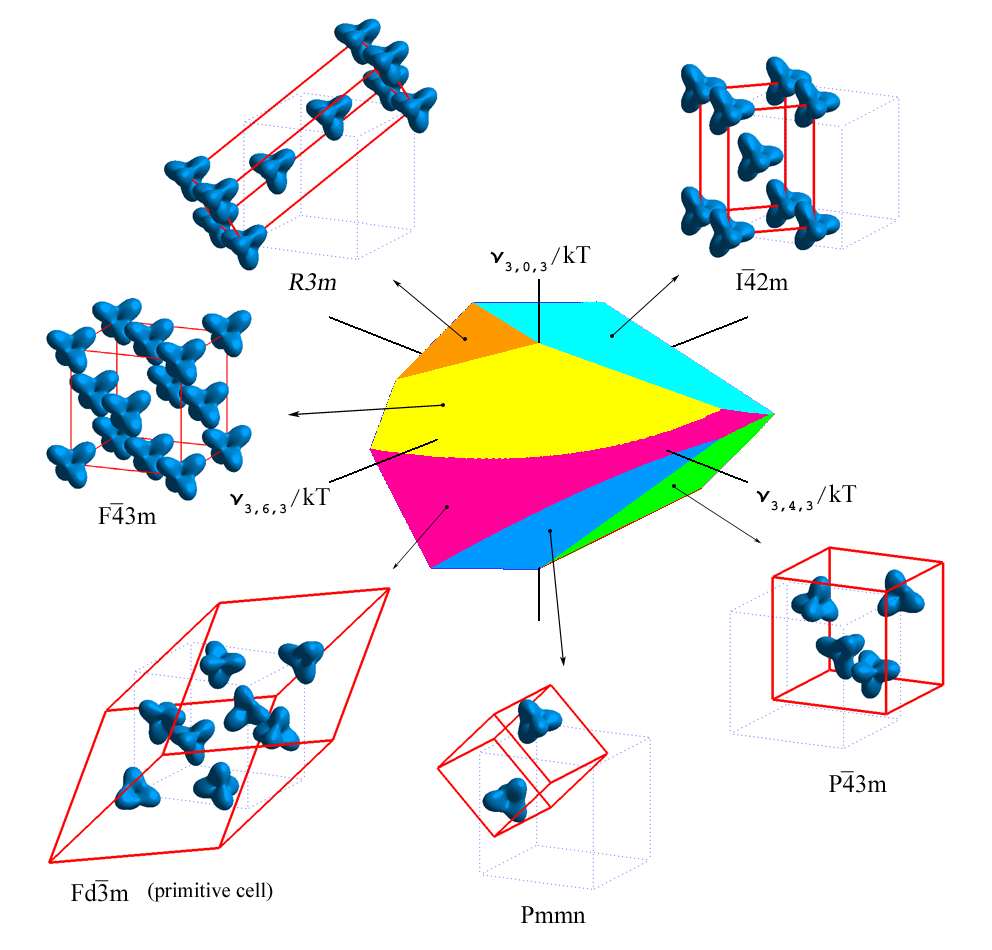
\includegraphics{figure1aII.eps}
%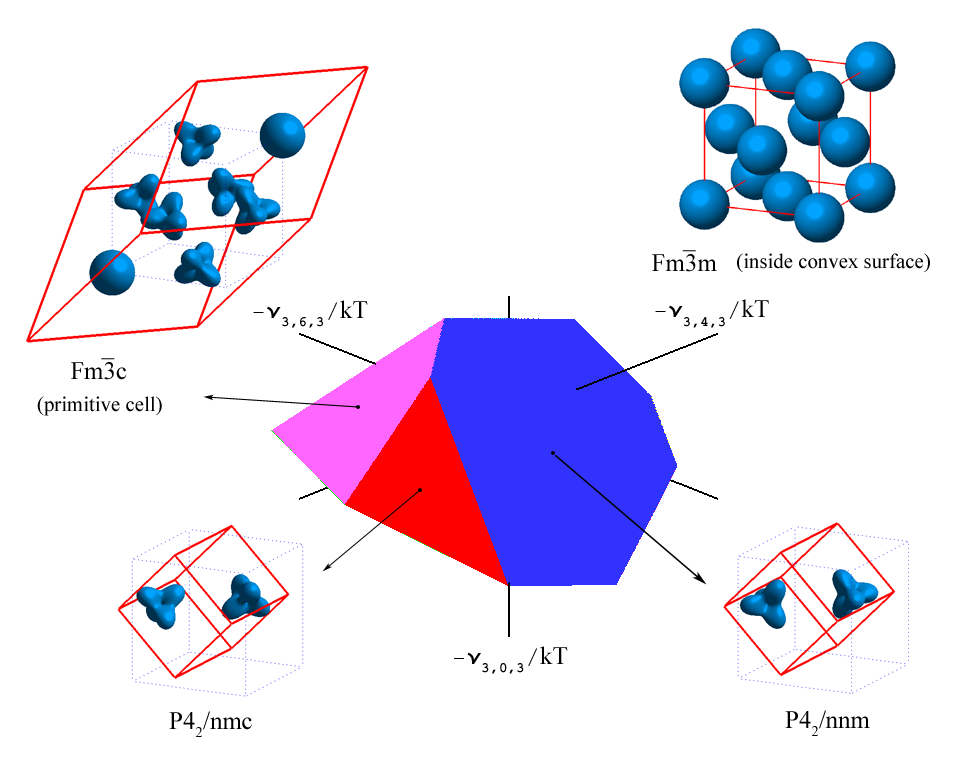
\includegraphics{figure1bII.eps}
\end{figure}

\pagebreak

\begin{figure}
\caption{$[\bar{1}\bar{1}\bar{1}]$ view of a GPD for tetrahedral molecules in
an fcc reference lattice. Some molecules such as
those in the $Fm\bar{3}m$ structure appear ``spherical" because of rapid molecular
reorientation. Reproduced with permission of the International
Union of Crystallography from \cite{Mettes04}} \label{gpd2}
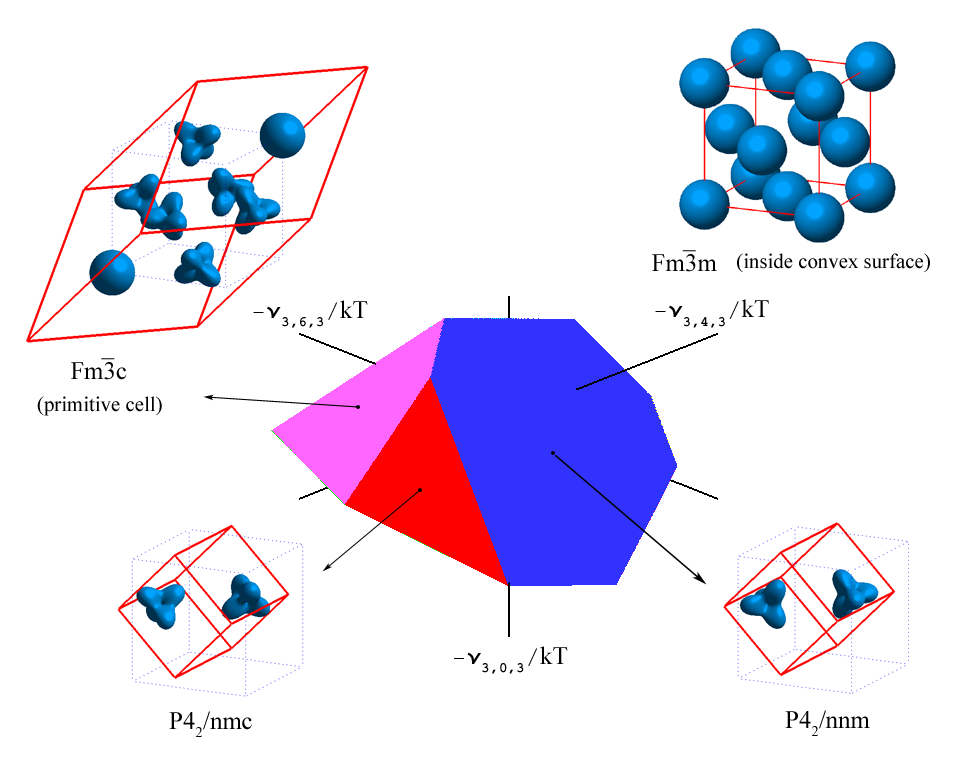
\includegraphics{figure1bII.eps}
\end{figure}

\pagebreak

\begin{table}%[!ht]
\caption{Presence of $O_h$ and $D_{3h}$ point group IRs for various
manifolds of SO(3). $O_h$ is the Wyckoff point group of the fcc,
bcc, and sc reference lattices. $D_{3h}$ is the Wyckoff point group
of the hcp reference lattice. The first occurrence of a given IR is
shown in bold.}\label{wyckoff_IRs}\small
\begin{tabular}{lll}\hline
$\ell_i$ & $O_h$ IRs &  $D_{3h}$ IRs \\
\hline
0 & $\mb{A_{1g}}$ & $\mb{A^\prime_1}$ \\
3 & $\mb{A_{2u}}+\mb{T_{1u}}+\mb{T_{2u}}$ &
$A^\prime_1+\mb{A^{\prime}_2}+\mb{E^\prime}+\mb{E^{\prime\prime}}$ \\
4 & $A_{1g}+\mb{E_{g}}+\mb{T_{1g}}+\mb{T_{2g}}$ &
$A^\prime_1+\mb{A^{\prime\prime}_1}+\mb{A^{\prime\prime}_2}+2E^\prime+E^{
\prime\prime}$\\
6 & $A_{1g}+\mb{A_{2g}}+E_g+T_{1g}+2T_{2g}$ &
$2A^\prime_1+A^{\prime\prime}_1+A^{\prime}_2+A^{\prime\prime}_2+2E^\prime+2E^{
\prime\prime}$ \\
7 & $A_{2u}+\mb{E_u}+2T_{1u}+2T_{2u}$ &
$A^\prime_1+A^{\prime\prime}_1+A^{\prime}_2+2A^{\prime\prime}_2+3E^\prime+2E^{
\prime\prime}$ `\\
8 & $A_{1g}+2E_g+2T_{1g}+2T_{2g}$ & \\
9 & $\mb{A_{1u}}+A_{2u}+E_u+3T_{1u}+2T_{2u}$ & \\
\hline
\end{tabular}
\end{table}

\pagebreak

\begin{table}%[!ht]
\caption{Group theoretical symmetry-breaking pathways of experimental lattices
for the fcc reference lattice. Classified by space group IR and order
parameter direction, each pathway shows the point group IR and
minimal manifold of SO(3) in Eq.~(\ref{re:eq:vij2}) required to
achieve it.  The order parameter directions are given in an abbreviated form in
the
notation of Stokes and
Hatch~\cite{Stokes02a}. The pathways, space
group IRs, order parameter directions, and point group IRs were computed using
ISOTROPY.
However, transitions belonging to a coupled IR between a high symmetry point and
line
are currently not a feature of ISOTROPY.  These entries have been marked with an
asterisk in
the table.} \label{pathwaysFCC}\tiny
\begin{tabular}{lllll}\hline
Pathway & S.~G.~IR & OP Dir. & P.~G.~IR & $\ell^{\mathrm{req'd}}$  \\
\hline
225a $\rightarrow$ 121a & $\Gamma_5^-$ & P1 & $T_{2u}$ & 3 \\

225a $\rightarrow$ 142a & $W_3$ & P2 & $T_{1g},A_{2u},E_{u}$ & 3 \\

225a $\rightarrow$ 114a & $X_2^-\oplus \Gamma_5^-$ & P1 $\oplus$ P1 &
$A_{2u},E_u \oplus
T_{2u}$ & 3 \\
& $X_3^+\oplus \Gamma_5^-$ &
P1 $\oplus$ P1 & $T_{1g} \oplus T_{2u}$ & 4 \\
& $X_2^- \oplus X_3^+$ & P1 $\oplus$ P1 & $A_{2u},E_{u} \oplus
T_{1g}$ & 4 \\

225a $\rightarrow$ 152b & $\Lambda_3$ (k=1/3) &  P1 &
$E_g,T_{1g},T_{2g},E_u,T_{1u},T_{2u}$ & 3 \\

225a $\rightarrow$ 15e (REKYUB) & $L_3^-$ & P7 & $E_u,T_{1u},T_{2u}$ & 3 \\

225a $\rightarrow$ 12i & $L_3^-$ & P2 & $E_u,T_{1u},T_{2u}$ & 3 \\

225a $\rightarrow$ 64d,f & $^*$\\

225a $\rightarrow$ 14e (MECKUA) & $\Gamma_3^+ \oplus L_3^-$ & P1 $\oplus$ C8 &
$E_g \oplus E_u,T_{1u},T_{2u}$ & 4 \\
& $\Gamma_3^+ \oplus X_5^-$ & C1 $\oplus$ S7 & $E_g \oplus T_{1u},T_{2u}$ & 4 \\
& $\Gamma_4^+ \oplus X_5^-$ & P1 $\oplus$ C11  & $T_{1g} \oplus T_{1u},T_{2u}$ &
4 \\
& & P1 $\oplus$ S7 \\
& $\Gamma_5^+ \oplus L_3^-$ & C2 $\oplus$ C8 & $T_{2g} \oplus E_u,T_{1u},T_{2u}$
& 4 \\
& $\Gamma_5^+ \oplus X_5^-$ & P1 $\oplus$ C11 & $T_{2g} \oplus T_{1u},T_{2u}$ &
4 \\
& & P1 $\oplus$ S7 & &  \\
& $L_2^+ \oplus L_1^-$ & P1 $\oplus$ P1 & $A_{2g},T_{1g} \oplus A_{1u},T_{2u}$ &
4 \\

& $L_2^+ \oplus L_3^-$ &  P1 $\oplus$ P7 & $A_{2g},T_{1g} \oplus
E_u,T_{1u},T_{2u}$ & 4 \\

& $L_2^+ \oplus X_2^-$ &  P1 $\oplus$ P1 & $A_{2g},T_{1g} \oplus A_{2u},E_u$ & 4
\\

& $L_2^+ \oplus X_3^-$ &  P1 $\oplus$ P1 & $A_{2g},T_{1g} \oplus E_u,T_{1u}$ & 4
\\

& $L_2^+ \oplus X_5^-$ &  P1 $\oplus$ P1 & $A_{2g},T_{1g} \oplus T_{1u},T_{2u}$
& 4 \\

& $L_3^+ \oplus L_1^-$ &  P7 $\oplus$ P1 & $E_g,T_{1g},T_{2g} \oplus
A_{1u},T_{2u}$ & 4 \\

& $L_3^+ \oplus L_3^-$ &  P7 $\oplus$ P7 & $E_g,T_{1g},T_{2g} \oplus
E_u,T_{1u},T_{2u}$ & 4 \\

& $L_3^+ \oplus X_2^-$ &  P7 $\oplus$ P1 & $E_g,T_{1g},T_{2g} \oplus A_{2u},E_u$
& 4 \\

& $L_3^+ \oplus X_3^-$ &  P7 $\oplus$ P1 & $E_g,T_{1g},T_{2g} \oplus E_u,T_{1u}$
& 4 \\

& $L_3^+ \oplus X_5^-$ &  P7 $\oplus$ P1 & $E_g,T_{1g},T_{2g} \oplus
T_{1u},T_{2u}$ & 4 \\

& $L_1^- \oplus L_3^-$ &  P1 $\oplus$ C8 & $A_{1u},T_{2u} \oplus
E_u,T_{1u},T_{2u}$ & 4 \\

& $L_1^- \oplus X_2^-$ &  P1 $\oplus$ P1 & $A_{1u},T_{2u} \oplus A_{2u},E_u$ & 4
\\

& $L_1^- \oplus X_3^-$ &  P1 $\oplus$ P1 & $A_{1u},T_{2u} \oplus E_u,T_{1u}$ & 4
\\

& $L_1^- \oplus X_5^-$ &  P1 $\oplus$ P1 & $A_{1u},T_{2u} \oplus T_{1u},T_{2u}$
& 4 \\

& $L_3^- \oplus X_2^-$ &  P7 $\oplus$ P1 & $E_u,T_{1u},T_{2u} \oplus A_{2u},E_u$
& 4 \\

& $L_3^- \oplus X_3^-$ &  P7 $\oplus$ P1 & $E_u,T_{1u},T_{2u} \oplus E_u,T_{1u}$
& 4 \\

& $L_3^- \oplus X_5^-$ &  P7 $\oplus$ P1 & $E_u,T_{1u},T_{2u} \oplus
T_{1u},T_{2u}$ & 4 \\

& $X_2^- \oplus X_5^-$ &  P1 $\oplus$ C11 & $A_{2u},E_u \oplus T_{1u},T_{2u}$ &
4 \\

& & P1 $\oplus$ S7 & &  \\

& $X_3^- \oplus X_5^-$ &  P1 $\oplus$ C11 & $E_u,T_{1u} \oplus T_{1u},T_{2u}$ &
4 \\

225a $\rightarrow$ 14e (TOHSUE) & $\Delta_5$ ($k=1/4$) & C7 &
$T_{1g},T_{2g},T_{1u},T_{2u}$ & 3 \\

225a $\rightarrow$ 15f,f,f,f & $C_2$ ($k_1=1/4,k_2=3/4$) & C18,C19 &
$A_{2g},E_g,T_{1g},T_{2g},$ & 3 \\
&  & & $A_{1u},E_u,T_{1u},T_{2u}$\\
\hline
\end{tabular}
\end{table}

\pagebreak

\begin{landscape}
\begin{table}%[!ht]
\caption{RP components for crystals of tetrahedral molecules in the
CSD.  The ``Identifier'' is a representative structure for a given structural
type.  The ``Multiplicity'' is the number of such structures in our dataset. The
$\ell_i$ truncation value and the presence, absence, or
proximity of a global minimum are indicated. The parameters
$\nu_{\ell_i,\ell,\ell_j}$ are indexed according to
Eq.~(\ref{re:eq:vij2}) and have been mapped to the unit hypersphere.}
\label{RPTop} \tiny
\begin{tabular}{llcccccccccccccccc}\hline
Identifier & Multi-& $\Delta$E & $\nu_{033}$ & $\nu_{044}$ & $\nu_{303}$ &
$\nu_{323}$ & $\nu_{343}$ & $\nu_{363}$ & $\nu_{314}$ & $\nu_{334}$
& $\nu_{354}$ & $\nu_{374}$ & $\nu_{404}$ & $\nu_{424}$ &
$\nu_{444}$ & $\nu_{464}$ & $\nu_{484}$ \\
& plicity & & & & & & & & & & & & & & & & \\
\hline
bcc\\
217a HXMTAM07 & 11 & 0.000 & - & 0.000 & 0.970 & 0.000 & 0.230 & -0.0790 & 0.000
& 0.000 & 0.000 & 0.000 & 0.000 & 0.000 & 0.000 & 0.000 & 0.000 \\
161a TCYMET & 1 & 0.007 & - & 0.355 & 0.303 & 0.380 & -0.017 & -0.130 & -0.213 &
0.084 & 0.331 & -0.116 & 0.409 & 0.496 & 0.075 & -0.138 & -0.089 \\
2i MEZDIE01 & 1 & 0.001 & - & -0.142 & 0.017 & -0.215 & 0.042 & 0.222 & 0.221 &
-0.314 & 0.483 & 0.230 & -0.287 & -0.309 & -0.019 & -0.158 & 0.495 \\
60c,d YIMWEW & 1 & -0.015 & - & 0.003 & 0.0 & 0.0 & 0.004 & 0.00 & 0.998 &
-0.007 & -0.059 & -0.008 & 0.002 & 0.0 & -0.002 & -0.010 & 0.009 \\
2iii OHABEE & 1 & 0.024 & - & 0.092 & -0.003 & -0.159 & -0.003 & 0.016 & -0.504
& 0.089 & -0.348 & 0.087 & -0.108 & -0.102 & -0.288 & -0.239 & 0.643 \\
\\
fcc\\
121a ZZZKDW01 & 1 & 0.000 & - & 0.000 & 0.431 & 0.316 & 0.267 & -0.802 & 0.000 &
0.000 & 0.000 & 0.000 & 0.000 & 0.000 & 0.000 & 0.000 & 0.000 \\
142a KUJSIR & 1 & 0.001 & - & 0.000 & -0.935 & -0.054 & 0.147 & -0.319 & 0.000 &
0.000 & 0.000 & 0.000 & 0.000 & 0.000 & 0.000 & 0.000 & 0.000 \\
114a ADAMAN08 & 2 & 0.018 & - & -0.035 & -0.007 & -0.292 & 0.000 & 0.023 & 0.061
& -0.046 & 0.191 & 0.053 & -0.056 & 0.584 & 0.185 & 0.055 & -0.698 \\
152b MTRETC10 & 1 & -0.080 & -  & -0.241 & 0.022 & -0.082 & 0.106 & -0.139 &
-0.909 & 0.002 & 0.109 & -0.244 & -0.001 & -0.045 & 0.012 & -0.067 & -0.003 \\
15e REKYUB & 1 & 0.003 & - & -0.210 & -0.001 & -0.359 & -0.011 & 0.031 & -0.157
& 0.135 & -0.463 & 0.379 & -0.209 & -0.445 & -0.340 & 0.157 & 0.208 \\
12i MECKOU & 1 & 0.000 & - & -0.258 & 0.006 & 0.781 & 0.028 & -0.058 & -0.216 &
-0.056 & -0.264 & 0.215 & -0.194 & 0.286 & 0.166 & 0.029 & 0.074 \\
64d,f METHANEIII & 1 & -0.238 & - & 0.112 & -0.010 & 0.017 & -0.020 & 0.006 &
0.001 & -0.022 & -0.002 & -0.014 & 0.097 & 0.060 & -0.772 & -0.483 & -0.379 \\
14e MECKUA & 1 & 0.005 & - & -0.123 & -0.070 & -0.103 & 0.161 & -0.744 & -0.240
& -0.084 & -0.209 & -0.345 & 0.008 & -0.251 & -0.056 & -0.305 & 0.060 \\
14e TOHSUE & 1 & -0.052 & - & 0.317 & -0.011 & -0.036 & 0.030 & -0.137 & 0.615 &
0.221 & -0.338 & 0.477 & 0.035 & -0.163 & -0.024 & -0.003 & 0.284 \\
15f,f,f,f CTBROM & 2 & -0.186 & - & 0.197 & 0.005 & -0.044 & -0.025 & -0.151 &
-0.687 & 0.291 & -0.284 & 0.486 & 0.037 & -0.062 & 0.038 & -0.077 & 0.222 \\
\\
hcp\\
165d DILWIE01 & 2 & -0.034 & -0.839 & 0.000  & 0.075 & 0.302 & 0.296 & -0.334 &
0.000  & 0.000  & 0.000  & 0.000  & 0.000  & 0.000  & 0.000  & 0.000 & 0.000 \\
147d ZIZHIZ & 1 & 0.000 & -0.793 & 0.000 & -0.040 & 0.203 & 0.083 & -0.568 &
0.000 & 0.000 & 0.000 & 0.000 & 0.000 & 0.000 & 0.000 & 0.000 & 0.000 \\
176h CUCZUV & 1 & 0.009 & 0.000 & 0.000  & -0.251 & -0.965 & 0.071 & -0.011 &
0.000  & 0.000  & 0.000  & 0.000  & 0.000  & 0.000  & 0.000  & 0.000  & 0.000 
\\
\\
sc\\
215a FOHCUA & 3 & 0.000 & - & 0.000 & 0.960 & 0.000 & 0.279 & -0.017 & 0.000 &
0.000 & 0.000 & 0.000 & 0.000 & 0.000 & 0.000 & 0.000 & 0.000 \\
120c YEMRIR & 1 & 0.016 & - & -0.102 & -0.111 & -0.167 & -0.439 & 0.077 & 0.403
& -0.487 & -0.078 & 0.281 & 0.169 & 0.056 & -0.071 & 0.449 & -0.167\\
\hline\\
\end{tabular}
\end{table}
\end{landscape}

\pagebreak

\begin{table}%[!ht]
\caption{Comparison of the cumulative number of parameters in
potential for a truncation at a given manifold for two truncation
strategies and three molecular point groups.}\label{tab:truncation}
\begin{tabular}{lllllllll}
\multicolumn{4}{c}{Direct Truncation} & &\multicolumn{4}{c}{$\ell$ sum
Truncation}\\
\cline{1-4}\cline{6-9}\\
$\ell_i$ & $C_1$ & $T_d$ & $I_h$ & & $\ell_i+\ell_j$ & $C_1$ &
$T_d$ & $I_h$\\
\cline{1-4}\cline{6-9}\\
0  & $^*$  & $^*$  & $^*$  & & 0  & $^*$  & $^*$ & $^*$ \\
1  & 3  & 0  & 0  & & 1  & 1  & 0 & 0 \\
2  & 60 & 0  & 0  & & 2  & 6  & 0 & 0 \\
3  &    & 5  & 0  & & 3  & 15 & 1 & 0 \\
4  &    & 10 & 0  & & 4  &    & 1 & 0 \\
6  &    &    & 8  & & 6  &    & 6 & 1 \\
10 &    &    & 19 & & 10 &    &   & 8 \\
\cline{1-4}\cline{6-9}\\
\end{tabular}
\\$^*$ There is one isotropic basis function for $\ell_i=\ell_j=0$ in
each case, but it does not drive orientational ordering.
\end{table}

\pagebreak

\begin{figure}%[!ht]
\scalebox{.38}{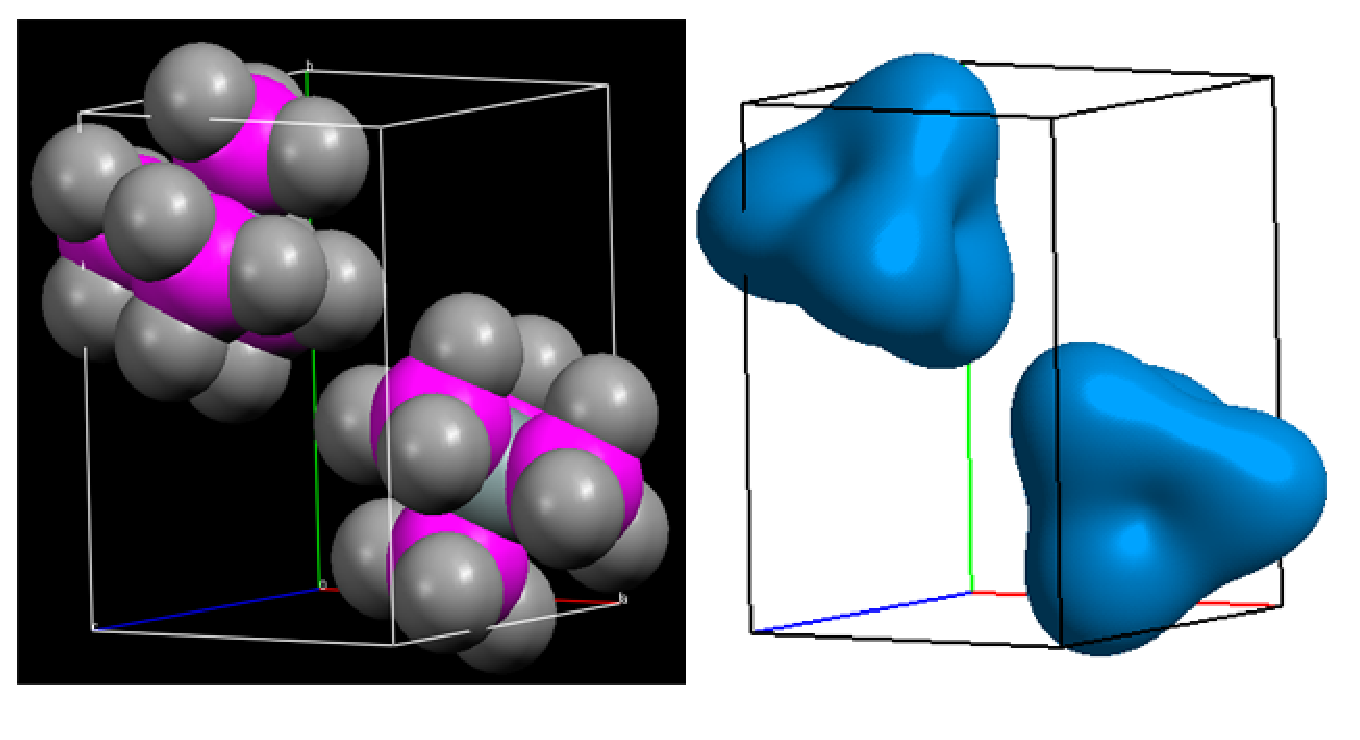
\includegraphics{mezdieCompareII.eps}}
\caption{Comparison of an experimental structure,
tetrakis(trimethystannyl)silane  [CSD structure MEZDIE01], which
crystallizes in space group 2 at Wyckoff point i with
arbitrarily-shaped tetrahedral figures whose orientation is
determined by orientational energy minimization with molecular
center of mass on an ideal bcc reference lattice.\label{compare}}
\end{figure}

\pagebreak

\appendix

\section{Detailed derivation of Eq.~\ref{re:eq:vij2}}
\label{derivation}

We choose to expand the potential using a complete set of
two-molecule basis functions that span the rotational space
$SO(3)$ parameterized by Euler angles $\mb{\omega}$ of molecule
$i,j$ and their intervening orientational space $S^2$
parameterized by solid angle
$\mb{\Omega}_{ij}=(\theta_{ij},\phi_{ij})$. Coupling two $SO(3)$
irreducible representations (IR's)
$D^{\ell_i}_{m_{i}n_{i}}(\mb{\omega}_i)$ and
$D^{\ell_j}_{m_{j}n_{j}}(\mb{\omega}_j)$ and a spherical harmonic
$C^\ell_m(\mb{\Omega}_{ij})$ gives
\begin{equation}
\label{Wbasis}W^{n_i n_j}_{\ell_i \ell \ell_j}=\sum_{m_imm_j}
\left(\begin{array}{ccc} \ell_i & \ell & \ell_j \\
m_i & m & m_j
\end{array}\right)D^{\ell_i}_{m_in_i}(\mb{\omega}_i)C^\ell_m(\mb{\Omega}_{ij})
D^{\ell_j}_{m_jn_j}(\mb{\omega}_j)
\end{equation}
where the explicit functional dependence of $C^\ell_m$ and
$D^{\ell_j}_{m_jn_j}$ has been dropped. This is done in the following manner,
where \cite{Varshalovich88}
\begin{eqnarray}
D_{mn}^{\ell}(\mb{\omega}_i)&=&\exp \left(-i m \alpha_i \right)
\, d_{mn}^{\ell}(\beta_i) \, \exp \left(-i n \gamma_i \right)\\
d_{mn}^{\ell}(\beta_i)&=&\sum_{k = \max(0,m-n )}^{\min( \ell+m,
\ell-n)} (-1)^k\nonumber\\
&&\!\!\!\!\!\!\!\!\!\!\!\!\times\frac{\left[(\ell+m)!\,(\ell-m)!\,(\ell+n)!\,
(\ell-n)!
\right]^{1/2}}{k!\,(\ell+m-k)!\,(\ell-n-k)!
\,(n-m+k)!}\nonumber \\
&&\!\!\!\!\!\!\!\!\!\!\!\!\times\left[\cos(\beta_i/2)\right]^{2\ell+m-n-2k}
 \left[\sin(\beta_i/2)\right]^{2k-m+n}\\
C_{m}^{\ell}(\mb{\Omega}_{ij})&=&\sqrt{\frac{4\pi}{2\ell+1}}Y_{m}^{\ell}(\mb{
\Omega}_{ij}),
\end{eqnarray}
we first couple angular basis functions of molecules $i$ and $j$
\begin{equation}
\label{angAB} A^{\ell_{(ij)}}_{m_{(ij)}}=
\sum_{m_im_j}C_{\ell_{i}m_{i},\ell_{j}m_j}^{\ell_{(ij)}m_{(ij)}}D^{\ell_i}_{
m_in_i}D^{\ell_j}_{m_jn_j}
\end{equation}
where $C_{\ell_{i}m_{i},\ell_{j}m_j}^{\ell_{(ij)}m_{(ij)}}$ is a
Clebsch-Gordan coefficient~\cite{Varshalovich88}.  Coupling
$A^{\ell_{(ij)}}_{m_{(ij)}}$ to the $C^\ell_m(\mb{\Omega}_{ij})$
and requiring the overall state to be a scalar $W$ we obtain
\begin{equation}
\label{angcoup}W^{n_i n_j}_{\ell_i \ell
\ell_j}=\sum_{mm_{(ij)}}C_{\ell\,m,\ell_{(ij)}m_{(ij)}}^{0
0}A^{\ell_{(ij)}}_{m_{(ij)}}C^\ell_m
\end{equation}
By definition the Clebsch-Gordan coefficient
$C_{\ell_1m_1,\ell_2m_2}^{\ell m}$ is zero unless $m_1+m_2=m$ so
that $m_2=-m_1$ if $m=0$. It is also zero unless
$|\ell_1-\ell_2|\leq \ell\leq \ell_1+\ell_2$, and since
$m_{1,2}\in\{\ell_{1,2}...-\ell_{1,2}\}$ this implies that
$\ell_1=\ell_2$. Thus $C_{\ell\,m,\ell_{(ij)}m_{(ij)}}^{0 0}$ in
Eq.~(\ref{angcoup}) simplifies to $C_{\ell m,\ell
\overline{m}}^{00}$. With the identity~\cite{Varshalovich88}
\begin{equation}
\label{coupid}C_{\ell m,\ell
\overline{m}}^{00}=\frac{(-1)^{\ell+m}}{\sqrt{2\ell+1}}
\end{equation}
we have
\begin{equation}
\label{inv}W^{n_i n_j}_{\ell_i \ell
\ell_j}=\sum_{m_imm_j}C_{\ell_i
m_i,\ell_jm_j}^{\ell\overline{m}}\frac{(-1)^{\ell+m}}{\sqrt{2\ell+1}}D^{\ell_i}_
{m_in_i}C^\ell_mD^{\ell_j}_{m_jn_j}
\end{equation}
Likewise using the identity~\cite{Varshalovich88}
\begin{equation}
\label{id}C^{\ell\overline{m}}_{\ell_im_i,\ell_jm_j}=(-1)^{\ell_i-\ell_j-m}\sqrt
{2\ell+1}\left(\begin{array}{ccc}
\ell_i & \ell_j & \ell \\ m_i & m_j & m \end{array}\right)
\end{equation}
gives
\begin{equation}
W^{n_i n_j}_{\ell_i \ell
\ell_j}=\sum_{m_imm_j}(-1)^{\ell_i-\ell_j+\ell}\left(\begin{array}{ccc}
\ell_i & \ell_j & \ell \\ m_i & m_j & m
\end{array}\right)D^{\ell_i}_{m_in_i}C^\ell_mD^{\ell_j}_{m_jn_j}.
\end{equation}
To remove the phase factor one may exploit the mirror symmetry of
the 3jm symbol
\begin{equation}
\left(\begin{array}{ccc} \ell_i & \ell_j & \ell \\ m_i & m_j & m
\end{array}\right)=(-1)^{\ell_i+\ell_j+\ell}\left(\begin{array}{ccc} \ell_i &
\ell & \ell_j \\ m_i & m & m_j
\end{array}\right)
\end{equation}
leaving
\begin{equation}
\label{appbasis}W^{n_i n_j}_{\ell_i \ell
\ell_j}=\sum_{m_imm_j}\left(\begin{array}{ccc} \ell_i & \ell & \ell_j \\
m_i & m & m_j
\end{array}\right)D^{\ell_i}_{m_in_i}C^\ell_m D^{\ell_j}_{m_jn_j}.
\end{equation}
Equation~(\ref{appbasis}) gives basis functions $W$ from Eq.~\ref{Wbasis}.
without any
symmetry adaptation.  The $W^{n_i n_j}_{\ell_i \ell \ell_j}$ form a complete set
of orthogonal IP
basis functions over the eight-dimensional space $SO(3)\times
S^2\times SO(3)$. Similar but slightly different constructions are given in the literature.\cite{Avoird80,Briels80,Stone84,Avoird94}

While $W^{n_i n_j}_{\ell_i \ell \ell_j}$ are
general, it is computationally advantageous to project out
the point group symmetry of the molecule and that of the Wyckoff
point. Appendix~\ref{Appx:proj} reviews our use of projection
operators which amount to matrix multiplication by a sparse
unitary matrix $S^{\ell_i}_{n_in_\sigma}$ where $\sigma$ refers to
a point group IR and $n_\sigma$ is a particular component of the
IR. For example, using projection operators for the molecular
point group yields symmetry-adapted matrix elements
\begin{eqnarray}
\label{eq:Tfunc}T^{\ell_i}_{m_i n_\sigma}(\mb{\omega}_i)&=&\sum_{n_i}D_{m_i
n_i}^{\ell_i}(\mb{\omega}_i)S^{\ell_i}_{n_in_\sigma}
\end{eqnarray}
which may be coupled to produce symmetry-adapted basis functions
\begin{equation}
\label{basis}F_{\ell_i\ell\ell_j}^{n_\sigma
n_\mu}=\sum_{m_imm_j}\left(\begin{array}{ccc} \ell_i & \ell & \ell_j \\
m_i & m & m_j
\end{array}\right)T^{\ell_i}_{m_i n_\sigma}(\mb{\omega}_i)
C^\ell_m(\mb{\Omega}_{ij}) T^{\ell_j}_{m_j n_\mu}(\mb{\omega}_j).
\end{equation}
With these basis functions the potential is
\begin{equation}
\label{eq:vij} V = \frac{1}{2}\sum_{ij} \sum_{\ell_i \ell \ell_j
n_\sigma n_\mu} \nu_{\ell_i\ell\ell_j}^{n_\sigma n_\mu}(r_{ij})
F_{\ell_i\ell\ell_j}^{n_\sigma
n_\mu}(\mb{\omega}_i,\mb{\Omega}_{ij},\mb{\omega}_j)
\end{equation}
where the one half avoids overcounting,
$\ell_i,\ell_j\in\mathbb{N}$, $|\ell_i-\ell_j|\leq\ell\leq
\ell_i+\ell_j$, and
$\nu_{\ell_i,\ell,\ell_j}^{n_\sigma,n_\mu}(r_{ij})$ are
coefficients which are a function of the distance $r_{ij}$ between
molecular centers. The full set of these in the potential is
termed $\mb{\nu}$. Subscripts $\sigma,\mu$ are a compound index
referring to multiple copies of the molecular point group unit IR
subduced in the $\ell_i,\ell_j$-th manifold of $SO(3)$ and
$n_\sigma,n_\mu$ is its dimension which is always
$n_\sigma,n_\mu=1$.  Point group IR subduction frequencies in
spherical harmonics are discussed elsewhere \cite{Bradley72}. All
other point group IR's do not have the full molecular symmetry and
so are zero to first order.

Projecting out Wyckoff point symmetry from the functions
$T^{\ell_i}_{m_i n_\sigma}$ gives rotator functions
\begin{equation}
\label{eq:rotfunc}U^{\ell_i}_{m_\tau n_\sigma}(\mb{\omega}_i)=\sum_{m_i
n_i}S^{\ell_i*}_{m_im_\tau}D_{m_i
n_i}^{\ell_i}(\mb{\omega}_i)S^{\ell_i}_{n_in_\sigma}.
\end{equation}
Expressing the potential using coupled rotator functions gives
\begin{equation}
\label{eq:vij2}V = \frac{1}{2}\sum_{ij}\sum_{\ell_i\ell_j m_\tau m_\rho
n_\sigma n_\mu} U^{\ell_i}_{m_\tau
n_\sigma}(\mb{\omega}_i)J_{m_\tau n_\sigma m_\rho n_\mu}^{\ell_i
\ell_j}(\mb{\Omega}_{ij})U^{\ell_j}_{m_\rho
n_\mu}(\mb{\omega}_j)
\end{equation}
where
\begin{eqnarray}
 J_{m_\tau n_\sigma m_\rho
n_\mu}^{\ell_i \ell_j}(\mb{\Omega}_{ij})&=&\sum_{\ell m_i m m_j}
\nu_{\ell_i,\ell,\ell_j}^{n_\sigma,n_\mu}(r_{ij})\left(\begin{array}{
ccc}
 \ell_i & \ell & \ell_j \\ m_i & m & m_j
\end{array}\right)\nonumber\\
&&\times S^{\ell_i}_{m_\tau m_i}C_{m}^{\ell} S^{\ell_j}_{m_\rho
m_j}
\end{eqnarray}
is a dimensionless coupling function. Subscripts $\tau,\rho$ are a
compound index referring to multiple copies of the Wyckoff point
group IR's subduced in the $\ell_i,\ell_j$-th manifold of $SO(3)$
and $m_\tau,m_\rho$ goes over the dimensions of each IR. 	

\pagebreak


\section{Projection Operators}
\label{Appx:proj}

Symmetries of the molecule and Wyckoff point of the crystal exist
within $D_{m_i,n_i}^{\ell_i}$ simultaneously and can be obtained
by applying projection operators
\cite{Bradley72}
\begin{equation}
P^{\tau}_{n_\tau n_\tau}=\sqrt{d_\tau/|G|}\sum_{g\in G}D^{\tau
*}_{n_\tau n_\tau}(g)\,g
\end{equation}
where $d_\tau$ is the dimension of the IR $\tau$ belonging to the
group $G$ of order $|G|$, $\mb{D}^\tau$ is the matrix onto which
the IR maps $g$, and subsequent orthonormalization is occasionally
required. We have used a slightly different normalization which
decreases the computation in this orthonormalization. Acting upon
the elements $D_{mn}^{\ell}$ gives
\begin{equation}
P^{\tau}_{n_\tau n_\tau}\circ D_{mn}^{\ell}=\sum_n
D_{mn}^{\ell}S_{nn_\tau}^\ell
\end{equation}
producing a linear combination with the symmetry of $\tau$.  The
coefficients $S_{nn_\tau}^\ell$ form a sparse unitary matrix.

%==============================================================================


\textbf{\begin{LARGE}Supplementary Material\end{LARGE}}

\pagebreak

\begin{table}%[!ht]
\caption{Group theoretical symmetry-breaking pathways of experimental lattices
from the
bcc reference lattice. Classified by space group IR and order
parameter direction, each pathway shows the point group IR and
minimal manifold of SO(3) in Eq.~(\ref{re:eq:vij2}) required to
achieve it.  The order parameter directions are given in an abbreviated form in
the
notation of Stokes and
Hatch~\cite{Stokes02a}.}\label{pathwaysBCC} \tiny
\begin{tabular}{lllll}\hline
Pathway & S.~G.~IR & OP Dir. & P.~G.~IR & $\ell^{\mathrm{req'd}}$  \\
\hline
229a $\rightarrow$ 217a & $\Gamma_2^-$ & P1 & $A_{2u}$ & 3 \\

229a $\rightarrow$ 161a & $H_5^- \oplus \Gamma_2^-$ & P3 $\oplus$ P1 & $T_{2u}
\oplus
A_{2u}$ & 3 \\
& $H_5^- \oplus \Gamma_4^-$ & P3 $\oplus$ P3 & $T_{2u} \oplus
T_{1u}$ &3 \\
& $H_5^- \oplus H_4^+$ & P3 $\oplus$ P3 & $T_{2u} \oplus T_{1g}$
& 4 \\
& $H_4^+ \oplus \Gamma_2^-$ & P3 $\oplus$ P1 & $T_{1g} \oplus A_{2u}$ & 4 \\
& $H_4^+ \oplus \Gamma_4^-$ & P3 $\oplus$ P3 & $T_{1g} \oplus T_{1u}$ & 4\\
& $H_5^- \oplus H_2^+$ & P3 $\oplus$ P1 & $T_{2u} \oplus A_{2g}$
& 6\\
& $H_2^+ \oplus \Gamma_4^-$ & P1 $\oplus$ P3 & $A_{2g} \oplus T_{1u}$ & 6 \\
& $H_1^- \oplus \Gamma_4^-$ & P1 $\oplus$ P3 & $A_{1u} \oplus
T_{1u}$ & 9 \\
& $H_1^- \oplus H_4^+$ & P1 $\oplus$ P3 & $A_{1u} \oplus T_{1g}$
& 9\\

229a $\rightarrow$ 2i (MEZDIE01) & $N_1^-\oplus\Gamma_4^+$ &
P1 $\oplus$ S1 & $A_{1u},E_u,T_{2u} \oplus T_{1g}$ & 4\\
& $N_1^-\oplus\Gamma_5^+$ & P1 $\oplus$ S1 & $A_{1u},E_u,T_{2u}
\oplus T_{2g}$ & 4\\
& $N_2^-\oplus\Gamma_4^+$ & P1 $\oplus$ S1 & $A_{2u},E_u,T_{1u}
\oplus T_{1g}$ & 4 \\
& $N_2^-\oplus\Gamma_5^+$ & P1 $\oplus$ S1 & $A_{2u},E_u,T_{1u}
\oplus T_{2g}$ & 4 \\
& $N_3^-\oplus\Gamma_4^+$ & P1 $\oplus$ S1 & $T_{1u},T_{2u} \oplus
T_{1g}$ & 4\\
& $N_3^-\oplus\Gamma_5^+$ & P1 $\oplus$ S1 & $T_{1u},T_{2u} \oplus
T_{2g}$ & 4\\
& $N_4^-\oplus\Gamma_4^+$ & P1 $\oplus$ S1 & $T_{1u},T_{2u} \oplus
T_{1g}$ & 4\\
& $N_4^-\oplus\Gamma_5^+$ & P1 $\oplus$ S1 & $T_{1u},T_{2u} \oplus
T_{2g}$ & 4\\

229a $\rightarrow$ 60c,d (YIMWEW) & $^*$\\

229a $\rightarrow$ 2iii & $H_4^-$ & S1 & $T_{1u}$ & 3\\
& H5- & S1 & $T_{2u}$ & 3\\
\hline
\end{tabular}
\end{table}

\pagebreak

\begin{table}%[!ht]
\caption{Group theoretical symmetry-breaking pathways of
experimental lattices for the hcp reference
lattice.}\label{pathwaysHCP}\tiny
\begin{tabular}{lllll}\hline
Pathway & S.~G.~IR & OP Dir. & P.~G.~IR & $\ell^{\mathrm{req'd}}$ \\
\hline
194c $\rightarrow$ 165d & $A_2$ & P3 & $A_2^\prime,A_1^\prime$ & 3 \\
194c $\rightarrow$ 147d & $\Gamma_3^+ \oplus \Gamma_2^+$ & P1$ \oplus$ P1 &
$A_2^{\prime\prime}\oplus A_2^\prime$ & 3 \\
& $\Gamma_4^+ \oplus \Gamma_2^+$ & P1$ \oplus$ P1 & $A_1^{\prime\prime}\oplus
A_2^\prime$ & 4 \\
& $\Gamma_4^+ \oplus \Gamma_3^+$ & P1$ \oplus$ P1 & $A_1^{\prime\prime}\oplus
A_2^{\prime\prime}$ & 4 \\
194c $\rightarrow$ 176h & $K_4$ & P1 & $E^\prime$ & 3 \\
\hline
\end{tabular}
\end{table}

\pagebreak

\begin{table}%[!ht]
\caption{Group theoretical symmetry-breaking pathways of
experimental lattices for the sc reference
lattice.}\label{pathwaysSC}\tiny
\begin{tabular}{lllll}\hline
Pathway & S.~G.~IR & OP Dir. & P.~G.~IR & $\ell^{\mathrm{req'd}}$  \\
\hline
221a $\rightarrow$ 215a & $\Gamma_2^-$ & P1 & $A_{2u}$ & 3 \\
221a $\rightarrow$ 120c & $R_5^-\oplus \Gamma_2^-$ & P1$ \oplus$ P1 & $T_{2u}
\oplus A_{2u}$  & 3 \\
& $R_4^+\oplus \Gamma_2^-$ & P1$ \oplus$ P1 & $T_{1g} \oplus A_{2u}$ & 4 \\
& $R_5^-\oplus R_4^+$ & P1$ \oplus$ P1 & $T_{2u} \oplus T_{1g}$  & 4 \\
& $R_4^+\oplus \Gamma_3^-$ & P1$ \oplus$ P1 & $T_{1g} \oplus E_u$  & 7 \\
& $R_5^-\oplus \Gamma_3^-$ & P1$ \oplus$ P1 & $T_{2u} \oplus E_u$  & 7 \\
\hline
\end{tabular}
\end{table}

Notes: 

(1) As these tables are not meant to be exhaustive enumerations but only
illustrative of the type of potentials necessary to find a given phase
transition, we have truncated listings for 161a, 2i (MEZDIE01), and 14e (MECKUA)
which have additional pathways similar to those shown. 

(2) Inasmuch as a different method was used in this work to choose an embedding
of the daughter lattice in the parent lattice than that used in
\cite{McClurg09}, the IRs inducing the phase transition from parent to daughter
may be different from \cite{McClurg09}.  This, of course, does not affect our
numerical results shown in Table \ref{RPTop}.

(3)  The pathways, space group IRs, order parameter directions, and point group
IRs were computed using ISOTROPY.
However, transitions belonging to a coupled IR between a high symmetry point and
line
are currently not a feature of ISOTROPY.  These entries have been marked with an
asterisk in
the table.

%have not been overly careful in our enumeration of coupled IR-induced pathways,
which increase rapidly in number and do not provide significant additional
information. For example, there may be a %few additional pathways which have
been omitted by oversight since ISOTROPY does not produce coupled IRs
automatically.  Rather, they must be found ``by hand''.  We note this since
certain %authors have made a practice of identifying such errors
\cite{Stokes84}.
\end{document}                    % DO NOT DELETE THIS LINE
%%%%%%%%%%%%%%%%%%%%%%%%%%%%%%%%%%%%%%%%%%%%%%%%%%%%%%%%%%%%%%%%%%%%%%%%%%%%%%

